\documentclass[12pt]{article}


%\usepackage{showkeys}
%\usepackage{drftcite}
\usepackage{exscale,relsize}
\usepackage{amsmath}
\usepackage{amsfonts}
\usepackage[colorlinks=true, linkcolor=blue]{hyperref}
\usepackage{amssymb}
\usepackage{calc}
\usepackage{theorem}
\usepackage{pifont}      % needed by dingautolist
\usepackage{array}
\usepackage{color}
\usepackage{enumerate}
\usepackage{bbm}
\usepackage{graphicx}
\usepackage{subcaption}
\usepackage{caption}

% \usepackage{amsthm}


% Hongda's packages
\usepackage{algpseudocode, algorithm}
\usepackage{mathtools}


% IF use the below packge, use `\printbibliography' to print out the bibliograph 
% For this one 
% 
% \usepackage[
%     backend=biber,
%     style=numeric,
%     sorting=nyt
% ]{biblatex}
% \addbibresource{references/PPM.bib}
% \addbibresource{references/NesterovMomentum.bib}
% \addbibresource{references/Books.bib}
% \addbibresource{references/BregmanDiv.bib}

% FORMATTING ===================================================================
\oddsidemargin -0.1cm
\textwidth  16.5cm
\topmargin  0.0cm
\headheight 0.0cm
\textheight 21.0cm
\parindent  4mm
\parskip    10pt
%\parskip    8pt
\tolerance  3000

% DRAFT FORMATTING =============================================================
% These are for todo notes, advise taken from 
% https://tex.stackexchange.com/questions/81666/extend-page-width-or-margin-for-todonotes-comments-or-other-package-comments
% \oddsidemargin=\dimexpr\oddsidemargin + 3cm\relax % DON'T USE

\ifthenelse{\boolean{draftmode}}{
    \evensidemargin=\dimexpr\evensidemargin  + 6cm\relax 
    \oddsidemargin=\dimexpr\oddsidemargin + 6cm\relax
    \paperwidth=\dimexpr \paperwidth + 12cm\relax 
    \marginparwidth=\dimexpr \marginparwidth  + 6cm\relax
    \paperheight=\dimexpr \paperheight + 6cm\relax
}{
    
}


% THEOREM AND ENVIRONMENTS.  ===================================================

%\newenvironment{deflist}[1][\quad]%
%{\begin{list}{}{\renewcommand{\makelabel}[1]{\textrm{##1~}\hfil}%
%\settowidth{\labelwidth}{\textrm{#1~}}%
%\setlength{\leftmargin}{\labelwidth+\labelsep}}}%requires macro calc.sty
%{\end{list}}
%\newtheorem{theorem}{Theorem}%[section]
\newtheorem{theorem}{Theorem}[section]
\newtheorem{lemma}[theorem]{Lemma}
\newtheorem{fact}[theorem]{Fact}
\newtheorem{corollary}[theorem]{Corollary}
\newtheorem{proposition}[theorem]{Proposition}
\newtheorem{definition}[theorem]{Definition}
\newtheorem{conjecture}[theorem]{Conjecture}
\newtheorem{observation}[theorem]{Observation}
\newtheorem{openprob}[theorem]{Open Problem}
\theoremstyle{plain}{\theorembodyfont{\rmfamily}
\newtheorem{assumption}[theorem]{Assumption}}
\theoremstyle{plain}{\theorembodyfont{\rmfamily}
\newtheorem{condition}[theorem]{Condition}}
\theoremstyle{plain}{\theorembodyfont{\rmfamily}}

% Removed due conflict with the algorithm environment. 
% \newtheorem{algorithm}[theorem]{Algorithm}}

\theoremstyle{plain}{\theorembodyfont{\rmfamily}
\newtheorem{example}[theorem]{Example}}
\theoremstyle{plain}{\theorembodyfont{\rmfamily}
\newtheorem{remark}[theorem]{Remark}}
\theoremstyle{plain}{\theorembodyfont{\rmfamily}
\newtheorem{application}[theorem]{Application}}

\def\proof{\noindent{\it Proof}. \ignorespaces}
%\def\endproof{\vbox{\hrule height0.6pt\hbox{\vrule height1.3ex%
%width0.6pt\hskip0.8ex\vrule width0.6pt}\hrule height0.6pt}}
%\numberwithin{equation}{section}
\def\endproof{\ensuremath{\quad \hfill \blacksquare}}

\renewcommand\theenumi{(\roman{enumi})}
\renewcommand\theenumii{(\alph{enumii})}
\renewcommand{\labelenumi}{\rm (\roman{enumi})}
\renewcommand{\labelenumii}{\rm (\alph{enumii})}

\numberwithin{equation}{section}



% These are Heniz's notations. 
\newcommand{\To}{\ensuremath{\rightrightarrows}}
\newcommand{\GX}{\ensuremath{\Gamma}}
\newcommand{\mal}{\ensuremath{\mathfrak{m}}}
\newcommand{\mumu}{\ensuremath{{\mu\mu}}}
\newcommand{\paver}{\ensuremath{\mathcal{P}}}
\newcommand{\ZZZ}{\ensuremath{{X \times X^*}}}
\newcommand{\RRR}{\ensuremath{{\RR \times \RR}}}
\newcommand{\todo}{\hookrightarrow\textsf{TO DO:}}

\newcommand{\emp}{\ensuremath{\varnothing}}
%\newcommand{\la}{\ensuremath{\langle}}
%\newcommand{\ra}{\ensuremath{\rangle}}
\newcommand{\infconv}{\ensuremath{\mbox{\small$\,\square\,$}}}
\newcommand{\pscal}{\ensuremath{\scal{\cdot}{\cdot}}}
\newcommand{\Tt}{\ensuremath{\mathfrak{T}}}
\newcommand{\YY}{\ensuremath{\mathcal Y}}
\newcommand{\XX}{\ensuremath{\mathcal X}}
\newcommand{\HH}{\ensuremath{\mathcal H}}
\newcommand{\XP}{\ensuremath{\mathcal X}^*}
\newcommand{\st}{\ensuremath{\;|\;}}
\newcommand{\zeroun}{\ensuremath{\left]0,1\right[}}

\newcommand{\lev}[1]{\ensuremath{\mathrm{lev}_{\leq #1}\:}}
\newcommand{\moyo}[2]{\ensuremath{\sideset{_{#2}}{}{\operatorname{}}\!#1}}
\newcommand{\pair}[2]{\left\langle{{#1},{#2}}\right\rangle}
%\newcommand{\scal}[2]{\left.\left\langle{#1}\:\right| {#2}  \right\rangle}
\newcommand{\scal}[2]{\langle{{#1},{#2}}\rangle}
\newcommand{\Scal}[2]{\left\langle{{#1},{#2}}\right\rangle}
%\newcommand{\scal}[2]{\braket{ {#1},{#2}}}

\newcommand{\yosida}{\ensuremath{ \; {}^}}
\newcommand{\exi}{\ensuremath{\exists\,}}
\newcommand{\GG}{\ensuremath{\mathcal G}}
\newcommand{\RR}{\ensuremath{\mathbb R}}
\newcommand{\SSS}{\ensuremath{\mathbb S}}
\newcommand{\CC}{\ensuremath{\mathbb C}}
\newcommand{\Real}{\ensuremath{\mathrm{Re}\,}}
\newcommand{\ii}{\ensuremath{\mathrm i}}
\newcommand{\RP}{\ensuremath{\left[0,+\infty\right[}}
\newcommand{\RPX}{\ensuremath{\left[0,+\infty\right]}}
\newcommand{\RPP}{\ensuremath{\,\left]0,+\infty\right[}}
\newcommand{\RX}{\ensuremath{\,\left]-\infty,+\infty\right]}}
\newcommand{\RXX}{\ensuremath{\,\left[-\infty,+\infty\right]}}
\newcommand{\KK}{\ensuremath{\mathbb K}}
\newcommand{\NN}{\ensuremath{\mathbb N}}
\newcommand{\nnn}{\ensuremath{{n \in \NN}}}
\newcommand{\thalb}{\ensuremath{\tfrac{1}{2}}}
\newcommand{\zo}{\ensuremath{{\left]0,1\right]}}}
\newcommand{\lzo}{\ensuremath{{\lambda \in \left]0,1\right]}}}
%\newcommand{\toppsepp}{\setlength{\partopsep}{-5pt}}
\newcommand{\menge}[2]{\big\{{#1} \mid {#2}\big\}}
\newcommand{\pfrac}[2]{\ensuremath{\mathlarger{\tfrac{#1}{#2}}}}


% MATH OPERATORS ===============================================================
% \newcommand{\monos}{\ensuremath{\mathcal M}}
\newcommand{\DD}{\operatorname{dom}f}
\newcommand{\IDD}{\ensuremath{\operatorname{int}\operatorname{dom}f}}
\newcommand{\CDD}{\ensuremath{\overline{\operatorname{dom}}\,f}}
\newcommand{\clspan}{\ensuremath{\overline{\operatorname{span}}}}
\newcommand{\cone}{\ensuremath{\operatorname{cone}}}
\newcommand{\dom}{\ensuremath{\operatorname{dom}}}
\newcommand{\closu}{\ensuremath{\operatorname{cl}}}
\newcommand{\cont}{\ensuremath{\operatorname{cont}}}
\newcommand{\mons}{\ensuremath{\mathcal{A}}}
\newcommand{\gra}{\ensuremath{\operatorname{gra}}}
\newcommand{\epi}{\ensuremath{\operatorname{epi}}}
\newcommand{\prox}{\ensuremath{\operatorname{Prox}_{\mu}}}
\newcommand{\hprox}{\ensuremath{\operatorname{prox}}}
\newcommand{\intdom}{\ensuremath{\operatorname{int}\operatorname{dom}}\,}
\newcommand{\inte}{\ensuremath{\operatorname{int}}}
\newcommand{\sri}{\ensuremath{\operatorname{sri}}}
\newcommand{\reli}{\ensuremath{\operatorname{ri}}}
\newcommand{\cart}{\ensuremath{\mbox{\LARGE{$\times$}}}}


\newcommand{\average}{\ensuremath{\mathcal{R}_{\mu}({\bf A},{\boldsymbol \lambda})}}
\newcommand{\averagebar}{\ensuremath{\mathcal{R}_{1}({\bf A},\bar{\lambda})}}
\newcommand{\averageonelambda}{\ensuremath{\mathcal{R}({\bf A},{\boldsymbol \lambda})}}
\newcommand{\averageonehalf}{\ensuremath{\mathcal{R}_{1}(A,1/2)}}
\newcommand{\averageinverse}{\ensuremath{\mathcal{R}_{\mu^{-1}}({\bf A}^{-1},{\boldsymbol \lambda})}}
\newcommand{\averageoneinverse}{\ensuremath{\mathcal{R}({\bf A}^{-1},{\boldsymbol \lambda})}}
\newcommand{\averagef}{\ensuremath{\mathcal{P}_{\mu}(f,\lambda)}}
\newcommand{\averagefone}{\ensuremath{\mathcal{P}_{1}(f,\lambda)}}
\newcommand{\averagefd}{\ensuremath{\mathcal{P}_{\mu}((f_{1},\ldots, f_{n}),(\lambda_{1},\ldots, \lambda_{n}))}}
\newcommand{\averagefik}{\ensuremath{\mathcal{P}_{\mu_{k}}((f_{1,k},\ldots,f_{n,k}),
(\lambda_{1,k},\ldots,\lambda_{n,k}))}}
\newcommand{\averagesub}{\ensuremath{\mathcal{R}_{\mu}(\partial f,\lambda)}}
\newcommand{\res}{\ensuremath{\mathcal{R}_{\mu}}}
\newcommand{\resmuk}{\ensuremath{\mathcal{R}_{\mu_{k}}}}
\newcommand{\newres}{\ensuremath{\mathcal{R}}}
\newcommand{\resmualpha}{\ensuremath{\mathcal{R}_{\alpha\mu}}}
\newcommand{\averageone}{\ensuremath{\mathcal{R}_{1}}}
\newcommand{\harm}{\ensuremath{\mathcal{H}(A,\lambda)}}
\newcommand{\arithmetic}{\ensuremath{\mathcal{A}(A,\lambda)}}

\newcommand{\WC}{\ensuremath{{\mathfrak W}}}
\newcommand{\SC}{\ensuremath{{\mathfrak S}}}
\newcommand{\card}{\ensuremath{\operatorname{card}}}
\newcommand{\bd}{\ensuremath{\operatorname{bdry}}}
\newcommand{\ran}{\ensuremath{\operatorname{ran}}}
\newcommand{\rec}{\ensuremath{\operatorname{rec}}}
\newcommand{\rank}{\ensuremath{\operatorname{rank}}}
\newcommand{\kernel}{\ensuremath{\operatorname{ker}}}
\newcommand{\conv}{\ensuremath{\operatorname{conv}}}
\newcommand{\segh}{\ensuremath{\operatorname{seg}}}
\newcommand{\boxx}{\ensuremath{\operatorname{box}}}
\newcommand{\clconv}{\ensuremath{\overline{\operatorname{conv}}\,}}
\newcommand{\cldom}{\ensuremath{\overline{\operatorname{dom}}\,}}
\newcommand{\clran}{\ensuremath{\overline{\operatorname{ran}}\,}}
\newcommand{\Nf}{\ensuremath{\nabla f}}
\newcommand{\NNf}{\ensuremath{\nabla^2f}}
\newcommand{\Fix}{\ensuremath{\operatorname{Fix}}}
\newcommand{\FFix}{\ensuremath{\overline{\operatorname{Fix}}\,}}
\newcommand{\aFix}{\ensuremath{\widetilde{\operatorname{Fix}\,}}}
\newcommand{\Id}{\ensuremath{\operatorname{Id}}}
\newcommand{\Max}{\ensuremath{\operatorname{max}}}
\newcommand{\Bb}{\ensuremath{\mathfrak{B}}}
\newcommand{\BB}{\ensuremath{\mathbb{B}}}
\newcommand{\Fb}{\ensuremath{\overrightarrow{\mathfrak{B}}}}
\newcommand{\Fprox}{\ensuremath{\overrightarrow{\operatorname{prox}}}}
\newcommand{\Bprox}{\ensuremath{\overleftarrow{\operatorname{prox}}}}
\newcommand{\Bproj}{\ensuremath{\overleftarrow{\operatorname{P}}}}
\newcommand{\Ri}{\ensuremath{\mathfrak{R}_i}}
\newcommand{\Dn}{\ensuremath{\,\overset{D}{\rightarrow}\,}}
\newcommand{\nDn}{\ensuremath{\,\overset{D}{\not\rightarrow}\,}}
\newcommand{\weakly}{\ensuremath{\,\rightharpoonup}\,}
\newcommand{\weaklys}{\ensuremath{\,\overset{*}{\rightharpoonup}}\,}
\newcommand{\gr}{\ensuremath{\operatorname{gra}}}
\newcommand{\g}{\ensuremath{\,\overset{g}{\rightarrow}}\,}
\newcommand{\p}{\ensuremath{\,\overset{p}{\rightarrow}}\,}
\newcommand{\e}{\ensuremath{\,\overset{e}{\rightarrow}}\,}
\newcommand{\Tbar}{\ensuremath{\overline{T}}}
\newcommand{\n}{\ensuremath{\,\overset{n}{\rightarrow}}\,}

\newcommand{\minf}{\ensuremath{-\infty}}
\newcommand{\pinf}{\ensuremath{+\infty}}
\renewcommand{\iff}{\ensuremath{\Leftrightarrow}}
% \renewcommand{\phi}{\ensuremath{\varphi}}
%\newcommand{\Real}{\ensuremath{\mathrm{Re}\,}}
\newcommand{\negent}{\ensuremath{\operatorname{negent}}}
\newcommand{\neglog}{\ensuremath{\operatorname{neglog}}}
\newcommand{\halb}{\ensuremath{\tfrac{1}{2}}}
\newcommand{\bT}{\ensuremath{\mathbf{T}}}
\newcommand{\bX}{\ensuremath{\mathbf{X}}}
\newcommand{\bL}{\ensuremath{\mathbf{L}}}
\newcommand{\bD}{\ensuremath{\boldsymbol{\Delta}}}
\newcommand{\bc}{\ensuremath{\mathbf{c}}}
\newcommand{\by}{\ensuremath{\mathbf{y}}}
\newcommand{\bx}{\ensuremath{\mathbf{x}}}
\newcommand{\bA}{{\bf A}}
\newcommand{\Other}{Indeterminate }
\newcommand{\other}{indeterminate }


%%% Raf's stuff  ===============================================================
\newcommand{\al}{\alpha}
\newcommand{\la}{\lambda}
\newcommand{\La}{\Lambda}
\newcommand{\pluss}{{\hskip1pt \raise1pt\vbox{\hrule width6pt \vskip1pt
\hrule width6pt}\kern-4pt{\lower1pt\hbox{\vrule height6pt \kern1pt\vrule
height6pt}}\hskip5pt}}
\newcommand{\timess}{\star}
\newcommand{\argmax}{\mathop{\rm argmax}\limits}
\newcommand{\argmin}{\mathop{\rm argmin}\limits}
\newcommand{\product}{\langle\cdot,\cdot\rangle}
\newcommand{\im}{\mathrm{Im}}
\newcommand{\multival}{\ensuremath{X\to 2^{X^*}}}
\newcommand{\SX}{\ensuremath{2^{X^*}}}

\newcommand{\inlinecode}[1]{\texttt{\footnotesize #1}}

\usepackage{listings} \lstset{basicstyle=\footnotesize\ttfamily,breaklines=true}
\usepackage{xcolor}
\lstdefinelanguage{Julia}%
  {morekeywords={abstract,break,case,catch,const,continue,do, else, elseif,%
      end, export, false, for, function, immutable, import, importall, if, in,%
      macro, module, otherwise, quote, return, switch, true, try, type, typealias,%
      using, while},%
   sensitive=true,%
   alsoother={$},%
   morecomment=[l]\#,%
   morecomment=[n]{\#=}{=\#},%
   morestring=[s]{"}{"},%
   morestring=[m]{'}{'},%
}[keywords,comments,strings]%
\lstset{%
    language         = Julia,
    basicstyle       = \ttfamily,
    keywordstyle     = \bfseries\color{blue},
    stringstyle      = \color{magenta},
    commentstyle     = \color{ForestGreen},
    showstringspaces = false,
}

% === TEMPLATE HOW TO USE ======
% To begine here is a list of things: 
% [ ]: Change title. 
% [ ]: Fill into the author names, affiliation and contact info. 
% [ ]: Fill in the abstract. 
% [ ]: Fill/change in AMS mathematics subject classification code, and the keywords. 

\title{
    {
        \fontfamily{ptm}\selectfont 
        First Order Nonsmooth Optimization: 
        Unifying Nesterov's acceleration and its applications
    }
}
\author{
    % \thanks{Department of Mathematics, I.K. Barber Faculty of Science,
    % The University of British Columbia, Kelowna, BC Canada V1V 1V7. 
    % E-mail:  \texttt{alto@mail.ubc.ca}.}~Hongda Li
    % \thanks{Department of Mathematics, I.K. Barber Faculty of Science,
    % The University of British Columbia, Kelowna, BC Canada V1V 1V7. 
    % E-mail:  \texttt{shawn.wang@ubc.ca}.}~ and~Author Name 2
    Hongda Li\\[3ex]\\ Department of Mathematics\\
	University of British Columbia,\\
	Okanagan Campus.
}
\date{\today}

\begin{document}
% \vspace{10ex}
% \vskip 8mm

\maketitle
\tableofcontents
\pagebreak



% \begin{abstract} 
%     \noindent
%     The research proposal focuses on the theories and practice in solving nonsmooth optimization. 
%     The theme of proposal highlight topics of interests that emphasize the computations and applications aspect of algorithms that exhibits both practical and theoretical importance. 
%     We summarize our ongoing research in unifying Nesterov type accelerated proximal gradient method and proposes our Free R-WAPG method. 
%     We survey literatures under the topic of Catalyst Meta Acceleration framework used in accelerating variance reduced methods in the settings of Data Science and Machine Learning. 
%     Furthermore, we present literatures and progress in topics such as Performance Estimation Problem, Inexact Proximal Point, acceleration without convexity. 
%     At the end there is a section summarizing a method we developed for tree species classifications using Sentinel-2 satellite remote sensing data using big data analytics by extract spectral signatures of ground vegetation covers. 


% \end{abstract}
% \noindent{\bfseries 2010 Mathematics Subject Classification:}
% Primary 65K10, 90c25, 90C30; Secondary 65Y20. 
% \noindent{\bfseries Keywords: } Non-convex Optimizations, Proximal Point. 


\section{Introduction}
    Let $\RR^n$ be the ambient space. We consider 
    \begin{align}
        \min_{x \in \RR^n} \left\lbrace
            F(x):= f(x) + g(x)
        \right\rbrace.
    \end{align}\label{eqn:additive-comp-obj}
    Unless specified, assume $f:\RR^n \rightarrow \RR$ is $L$-Lipscthiz smooth $\mu \ge 0$ strongly convex and $g:\RR^n \rightarrow \overline \RR$ is convex. 
    This type of problem is referred to as additive composite problems in the literature. 
    \par
    Our ongoing research concerns accelerated proximal gradient type method for solving (\ref{eqn:additive-comp-obj}). 
    In the expository writing by Walkington \cite{noel_nesterovs_nodate}, a variant for of accelerated gradient method for strongly convex function $f$ is discussed. 
    We had some lingering questions after reading it. 
    \begin{enumerate}
        \item Do there exist a unified description for the convergence for both variants of the algorithms?
        \item Is it possible to attain fast convergence rate without knowledge about the strong convexity of function $f$?
        \item Is it possible to describe the convergence of function value for momentum sequences that are much weaker than the Nesterov's rule? 
    \end{enumerate}
    The good news is we have definitive answers for all questions in our draft paper. 
    \par
    In this proposal we explore the Goldilocks zones between theories and practices of optimization algorithms. 
    Our topics are Nesterov's acceleration and the method of Catalyst Acceleration which is realization of the theories of Nesterov's acceleration and inexact proximal point method in the settings of variance reduced method in Machine Learning. 
    \par
    \textbf{Organizations now follows.} 
    In section \ref{sec:unify-nes-acceleration} we propose the method of ``Relaxed Weak Accelerated Proximal Gradient (R-WAPG)'' unifies the convergence results of several Euclidean variants of Accelerated Proximal Gradient (APG) method in the literatures and in addition to claiming the convergence when the momentum sequence doesn't follow the Nesterov's update rule. 
    \par
    Section \ref{sec:free-rwapg} gives an algorithm which is a reformulation of R-WAPG and, it achieves competitive convergence results (\ref{eqn:additive-comp-obj}) without restarting and knowing parameter $L, \mu$ in prior. 
    Numerical experiments are presented and potential future direction of research is given by the end of the section for the R-WAPG framework. 
    \par
    Section \ref{sec:catalyst} reviews the series of papers \cite{lin_universal_2015,lin_catalyst_2018,paquette_catalyst_2018} on Catalyst Meta Acceleration for First Order Variance Reduced Methods. 
    The content complements report completed for MATH 590 Fall Winter 2024. 
    The end of Section \ref{sec:catalyst} points out potential future direction of research of Catalyst Acceleration. 


    
\section{Preliminaries}
    This section contains the basics of contents from convex optimization, and variational analysis. 
    Throughout, we adopt the notation $\overline \RR := \RR \cup \{\infty, -\infty\}$. 
    \subsection{Fundamentals in non-convex analysis}
        Let the ambient space be $\RR^n$ equipped with inner product $\langle \cdot, \cdot\rangle$ and 2-norm $\Vert \cdot\Vert$. 
        Let $O$ be an open subset of $\RR^n$, the weakest assumption we make for objective function $F: O \subseteq \RR^n \rightarrow \RR$ of an optimization problem is local Lipschitz continuity. 
        The assumption of local Lipschitz continuity is weak enough to describe most problems in applications, and strong enough to avoid most pathologies in analysis. 

        \begin{definition}[Local Lipschitz continuity]
            Let $F: O \subseteq \RR^n \rightarrow \RR$ be Locally Lipschitz and $O$ is an open set. 
            Then for all $\bar x \in O$, there exists a Neighborhood: $\mathcal N(\bar x)$ and $K \in \RR$ such that for all $x, y \in \mathcal N(\bar x)$: $|F(x) - F(y)| \le K \Vert x - y\Vert$. 
        \end{definition}
        \begin{definition}[Regular subgradient]
            Let $F: O \subseteq \RR^n \rightarrow \RR$ be locally Lipschitz and $\bar x \in O$. 
            The regular subdifferential at $\bar x$ is defined as 
            \begin{align*}
                \widehat \partial F(\bar x) := 
                \left\lbrace
                    v \in \RR^n \left| \; 
                        \liminf_{\bar x \neq x\rightarrow \bar x}
                        \frac{F(x) - F(\bar x) - \langle v, x - \bar x\rangle}{\Vert x - \bar x\Vert} 
                        \ge 0
                    \right.
                \right\rbrace. 
            \end{align*}
        \end{definition}
        \begin{remark}
            Definition taken from Definition 4.3.1 from 
            Pang, Cui's book \cite{ying_modern_2021}
        \end{remark}
        \begin{definition}[Limiting subgradient]
            Let $F: O \subseteq \RR^n \rightarrow \RR$ be locally Lipschitz and $\bar x \in O$. 
            The limiting subdifferential at $\bar x$ is defined as 
            \begin{align*}
                \partial F(\bar x) := 
                \left\lbrace
                    v \in \RR^n \left| \; 
                        \exists x_k \rightarrow \bar x, v_k \rightarrow v: 
                        v_k \in \widehat \partial F(x_k) \;\forall k \in \mathbb N
                    \right.
                \right\rbrace. 
            \end{align*}
        \end{definition}
        \begin{remark}
            Definition taken from Definition 4.3.1 from
            Pang, Cui's book \cite{ying_modern_2021}
        \end{remark}
        \begin{definition}[Weakly convex function]
            $F: \RR^n \rightarrow \overline \RR$ is $\mu$ weakly convex if and only if $F + \frac{\mu}{2}\Vert \cdot\Vert^2$ is convex. 
        \end{definition}
        \begin{definition}[Bregman divergence]
            Let $F: O \subseteq \RR^n \rightarrow \RR$ be a differentiable function. 
            Then the Bregman divergence of $F$ is defined as: 
            \begin{align*}
                D_F(x, y): O \times \dom(\partial F) \rightarrow \RR
                := F(x) - F(y) - \langle \nabla F(y), x - y\rangle. 
            \end{align*}
        \end{definition}
    \subsection{Fundamentals in convex analysis}
        This section introduces the classics and basics of convex analysis. 
        Define $F$ to be closed, proper and convex in this section. 
        When $F$ is convex, the limiting subgradient and the regular subgradient reduced to the following: 
        \begin{align*}
            \partial F(x) = \left\lbrace
                v \in \RR^n \left|\; 
                    \forall y \in \RR^n\; :  F(y) - F(x)  \ge \langle v, y - x\rangle
                \right.
            \right\rbrace. 
        \end{align*}
        A convex function is locally Lipschitz in the relative interior of its domain, denoted as $\reli(\dom(F))$. 
        So it has 
        $\reli(\dom F)\subseteq \dom(\partial F) \subseteq \dom F$.
        See Rockafellar's book \cite[pg 82]{rockafellar_convex_1997}. 
        \par
        When we say $F:\RR^n \rightarrow \RR$ is $L$ Lipschitz smooth function, it means that there exists $L$ such that for all $x\in \RR^n, y \in \RR^n$, it has: 
        \begin{align*}
            \Vert \nabla F(x) - \nabla F(y)\Vert \le L \Vert x - y\Vert. 
        \end{align*}
        When $F$ convex, then it has descent lemma: 
        \begin{align*}
            (\forall x \in \RR^n)(\forall y \in \RR^n): 0 \le 
            F(x) - F(y) - \langle \nabla f(y), x - y\rangle \le \frac{L}{2}\Vert x - y\Vert^2. 
        \end{align*}
        The converse holds under convexity as well. 
        The definitions that follow narrow things further. 
        \begin{definition}[Strong convexity]\label{def:s-cnvx}
            A function $F:\RR^n \rightarrow \overline \RR$ is $\mu \ge 0$ strongly convex if and only if for all $y \in \dom(\partial F)$, $x\in \RR^n$: 
            \begin{align*}
                (\forall v \in \partial F(x))\quad 
                F(x) - F(y) \ge \langle v, x - y\rangle + \frac{\mu}{2}\Vert x - y\Vert^2. 
            \end{align*}
        \end{definition}
        \begin{lemma}[Quadratic growth from strong convexity]\label{lemma:q-growth}
            If $F$ is $\mu \ge 0$ strongly convex, $\bar x$ is a minimizer of $F$. 
            Then for all $x \in \RR^n$
            \begin{align*}
                F(x) - F(\bar x) \ge \frac{\mu}{2}\Vert x - \bar x\Vert^2. 
            \end{align*}
        \end{lemma}
        \begin{remark}
            The minimizer is unique whenever $\mu > 0$. 
            For contradiction, assume $x \neq \bar x$ is another minimizer, then $F(x) \neq F(\bar x)$, which is a direct contradiction. 
            This condition is called quadratic growth over the set of minimizer, it is much weaker than strong convexity. 
        \end{remark}
        
        \subsubsection{Smooth, nonsmooth additive composite}\label{sssec:additive-composite}
            This section zooms in further into the case of additive composite objective $F:= f + g$. 
            Assume $f$ is $L$ Lipschitz smooth and $\mu \ge 0$ strongly convex, $g: \RR\rightarrow \overline \RR$ is closed convex. 
            For all $\beta \ge 0$, define the proximal gradient, proximal point model functions as a mapping of $\RR^n \times \RR^n \rightarrow \overline \RR$: 
            \begin{align*}
                \widetilde{\mathcal M}^{\beta^{-1}}_F
                (x; y)
                &:= 
                g(x) + f(y) + \langle \nabla f(y), x - y\rangle
                + \frac{\beta}{2}\Vert x - y\Vert^2,
                \\
                \mathcal M^{\beta^{-1}}_F(x; y) 
                &:= F(x) + \frac{\beta}{2}\Vert x - y\Vert^2.
            \end{align*}
            Under the assumptions of this section, $\widetilde {\mathcal M}_F^{\beta^{-1}} (\cdot; y),  {\mathcal M}_F^{\beta^{-1}}(\cdot;y )$ are both $\beta + \mu$ strongly convex. 
            \begin{definition}[Proximal gradient operator]\label{def:proximal-gradient-operator}
                % Take $F := f + g$ where $g: \RR^n \rightarrow \overline \RR$ as defined in this section. 
                Define the proximal gradient operator $T_L$ on all $y \in \RR^n$: 
                \begin{align*}
                    T_L y := \argmin_{x \in \RR^n} \left\lbrace
                        g(x) + f(y) + \langle \nabla f(y), x - y\rangle 
                        + \frac{L}{2}\Vert x- y \Vert^2
                    \right\rbrace. 
                \end{align*}
            \end{definition}
            \begin{remark}
                Under the assumption of this section, the mapping $T_L$ is a single-valued mapping on $\RR^n$ and it's  a $3/2$ averaged operator. 
            \end{remark}
            \begin{definition}[Gradient mapping operator]\label{def:gradient-mapping-operator}
                % Take $F := f + g$ as defined in this section. 
                Define the gradient mapping operator $\mathcal G_L$ on all $y \in \RR^n$: 
                \begin{align*}
                    \mathcal G_L (y):= L(y - T_L y). 
                \end{align*}
            \end{definition}
            % \begin{lemma}[Proximal gradient model function]\;\\
            %     % Take $\widetilde{\mathcal M}^{L^{-1}}, \mathcal M^{L^{-1}}$ as defined in this section, 
            %     For all $x \in \RR^n$, $\beta > 0$, it has: 
            %     \begin{align*}
            %         \widetilde{\mathcal M}^{\beta^{-1}}_F(x; y)
            %         &= 
            %         \mathcal M^{\beta^{-1}}_F(x; y)- D_f(x, y).
            %     \end{align*}
            % \end{lemma}
            % \begin{lemma}[A favorable property of gradient mapping]
            %     % Take $F:= f + g$ as defined in this section. 
            %     For any $x \in \RR^n$. 
            %     Then there exists $v \in \partial g(T_L x)$ such that $\mathcal G_L (x) = v + \nabla f(x)$. 
            % \end{lemma}
            \begin{lemma}[The proximal gradient inequality]\label{thm:prox-grad-ineq}
                % Take $F:= f + g$ as defined in this section. 
                For all $y \in \RR^n$, $x \in \RR^n$, it has: 
                \begin{align*}
                    (\forall x \in \RR^n)\quad 
                    F(x)  - F(T_Ly) - \langle L(y - T_Ly), x - y\rangle
                    - \frac{\mu}{2}\Vert x - y\Vert^2 - \frac{L}{2}\Vert y - T_Ly\Vert^2 
                    &\ge 0. 
                \end{align*}
            \end{lemma}
            \begin{remark}
                This lemma is proved in our draft paper. 
            \end{remark}

    \subsection{Nesterov's estimating sequence technique}
        The derivation of APG was originally conceived by Nesterov's estimating sequence technique. 
        We emphasize that the technique derives the algorithm and proves its convergence rate. 
        \par
        The method is widespread in the literatures, and the ideas behind it are tremendously useful. 
        Güler \cite{guler_new_1992} used it to derive an accelerated proximal point method, which was instrumental to develop the Catalyst Acceleration framework. 
        Nesterov \cite{nesterov_accelerating_2008} used it to conceive the accelerated cubic regularized Newton's method. 
        In (6.1.19) of Nesterov's book \cite{nesterov_lectures_2018}, it's used to derive a method of accelerated mirror descent. 
        Finally, in Geovani N. et al \cite{grapiglia_accelerated_2019}, they used it to derive an accelerated Newton's method for convex composite objective function. 
        \par
        The definition of the estimating sequence that follows is based on our own understanding of the estimating sequence. 
        \begin{definition}[Nesterov's estimating sequence]\label{def:nes-est-seq}
            For all $k \ge 0$, let $\phi_k : \RR^n \rightarrow\RR$ be a sequence of functions. 
            We call this sequence of functions a Nesterov's estimating sequence when it satisfies conditions: 
            \begin{enumerate}
                \item There exists another sequence $(x_k)_{k \ge 0}$ such that for all $k \ge 0$ it has $F(x_k) \le \phi_k^*: =\min_{x}\phi_k(x)$. 
                \item There exists a sequence of $(\alpha_k)_{k \ge 0}$ where $\alpha_k \in (0, 1)\; \forall k \ge0 $ such that for all $x \in \RR^n$ it has $\phi_{k + 1}(x) - \phi_k(x) \le - \alpha_k(\phi_k(x) - F(x))$. 
            \end{enumerate}
        \end{definition}
        % \begin{observation}
        %     In general, identifying the sequence $(x_k)_{k \ge 0}$ is non-trivial. 
        %     But in case it can be found, the method of estimating sequence gives us the convergence rate described by the sequence $(\alpha_k)_{k \ge 0}$, and a candidate algorithm that generates the sequence $(x_k)_{k \ge 0}$. 
        %     It's two birds with one stone. 
        %     \par 
        %     If we define $\phi_k$, $\Delta_k(x) := \phi_k (x) - F(x)$ for all $x \in \RR^n$ and assume that $F$ has minimizer $x^*$. 
        %     Then observe that $\forall k \ge 0$:  
        %     \begin{align*}
        %         (\forall x \in \RR^n) \; \Delta_k(x) 
        %         &= \phi_k(x) - F(x) \ge \phi_k^* - F(x), 
        %         \\
        %         x = x_k\implies 
        %         \Delta_k(x_k) 
        %         &\ge 
        %         \phi_k^* - F(x_k) \ge 0;
        %         \\
        %         x = x_* \implies 
        %         \Delta_k(x_*)
        %         &\ge \phi_k^* - F_* \ge F(x_k) - F_* \ge 0. 
        %     \end{align*}
        %     The function $\Delta_k(x)$ is non-negative at points: $x_*, x_k$.
        %     We can derive the convergence rate of $\Delta_k(x^*)$ because (ii) says $\forall x \in \RR^n$: 
        %     \begin{align*}
        %         \phi_{k + 1}(x) - \phi_k(x) = \phi_{k + 1}(x) - F(x) - (\phi_k(x) - F(x))
        %         &\le - \alpha_k (\phi_k(x) - F(x))
        %         \\
        %         \iff
        %         \Delta_{k + 1}(x) - \Delta_k(x) &\le
        %         - \alpha_k\Delta_k(x)
        %         \\
        %         \iff 
        %         \Delta_{k + 1}(x) 
        %         &\le 
        %         (1 - \alpha_k)\Delta_k(x). 
        %     \end{align*}
        %     Unrolling the above recursion it yields: 
        %     \begin{align*}
        %         \Delta_{k + 1}(x) &\le 
        %         (1 - \alpha_k)\Delta_k(x) \le \cdots \le 
        %         \left(
        %             \prod_{i = 0}^k(1 - \alpha_i)
        %         \right)\Delta_0(x). 
        %     \end{align*}
        %     Finally, by setting $x = x^*$, $\Delta_k(x^*)$ is non-negative and using (i) it gives: 
        %     \begin{align*}
        %         F(x_k) - F(x^*) \le \phi_k^* - F(x^*) \le \Delta_k(x^*) = \phi_k(x^*) - F(x^*) \le \left(\prod_{i = 0}^k(1 - \alpha_i)\right)\Delta_0(x^*).
        %     \end{align*} 
        % \end{observation}
        

\section{Unifying NAG, and weakening the sequence assumption for convergences}\label{sec:unify-nes-acceleration}
    This section is based on our unpublished draft paper. 
    The Nesterov's acceleration scheme which was originally proposed in 1983 \cite{nesterov_method_1983} is a celebrated first order method for solving the minimization problem. 
    Initialize $x_1 = y_1$ and $t_0 = 1$, the algorithm finds $(x_k)_{k \ge 1}$ for all $k \ge 1$ by: 
    \begin{align}
        & x_{k + 1} = y_k - L^{-1}\nabla F(y_k), 
        \\
        & t_{k + 1} = 1/2\left(1 + \sqrt{1 + 4t_{k}^2}\right), 
        \\
        & \theta_{k + 1} = (t_{k} - 1)/t_{k + 1}, 
        \\
        & y_{k + 1} = x_{k + 1} + \theta_{k + 1}(x_{k + 1} - x_k). 
    \end{align}\label{eqn:example_algorithm}
    If the minimizer $x^*$ exists, then the optimality gap $F(x_k) - F(x^*)$ decreases at a rate of $\mathcal O(1/k^2)$, a faster rate compared to gradient descent which is $\mathcal O(1/k)$. 
    It's consider optimal in some sense and see Chapter 2 of Nesterov's book \cite{nesterov_lectures_2018} for details. 
    \subsection{Contributions}
        Inspired specifically by the technique of Nestrov's estimating sequence \cite{nesterov_lectures_2018}, firstly we present a unified framework of Accelerated Proximal Gradient (APG) which we call Relaxed Weak Accelerated Proximal Gradient (R-WAPG) in Section \ref{sec:rwapg-formulation-convergence}.
        It has the ability to upper bound $F(x_k) - F(x^*)$ for sequences $(t_k)_{k \ge 0}$ that follows a rule much weaker than Nesterov's update rule. 
        In addition to a convergence claim of $F(x_k)- F(x^*)$ for a much more flexible choice of $(t_k)_{k \ge 1}$. 
        Secondly, we present an alternative to restarting that performs well empirically inspired by a small detail in the convergence proof of R-WAPG. 
        It also has descriptive power to describe several variants of FISTA in the literatures.  
        \par
        Our contributions are two folds, theoretical and practical. 
        Our results are based the assumption $F = f + g$ where $g:\RR^n \rightarrow \overline\RR$ is convex proper and closed, and $f$ is an $L$-Lipschitz smooth and $\mu \ge 0$ strongly convex function. 
        \par
        \textbf{A summary of our main results follow. } 
        Nesterov's acceleration extrapolate $y_{k + 1} = x_{k + 1} + \theta_{k + 1}(x_{k + 1} - x_k)$ where $\theta_{k + 1} = (t_{k} - 1)/t_{k + 1} \in (0, 1)$ is the ``momentum''. 
        The choices for $\theta_k$ varies for different variants of the accelerated proximal gradient algorithm. 
        In Chambolle, Dossal \cite{chambolle_convergence_2015}, it has $t_k = (n + a - 1)/a$ for all $a > 2$ which gives weak convergence of the iterates $x_k$ in Hilbert space. 
        In Chapter 10 of Beck's Book \cite{beck_first-order_2017}, a variant called V-FISTA can achieve the faster linear convergence rate: $\mathcal O((1 - \sqrt{\mu/L})^k)$ on the optimality gap for $\mu > 0$ strongly convex $F$. 
        V-FISTA has $\theta_t = (\sqrt{\kappa} - 1)/(\sqrt{\kappa} + 1)$ where $\kappa = \mu/L$. 
        \par
        We relax the traditional choice of the sequence $\theta_k$ in Equation \ref{eqn:example_algorithm} and showed an upper bound of the optimal gap. 
        Let $(\alpha_k)_{k \ge0}, (\rho_k)_{k \ge 0}$ be two sequences that satisfy
        \begin{align*}
            \alpha_0 &\in (0, 1], 
            \\
            \alpha_k &\in (\mu/L, 1) \quad (\forall k \ge 1), 
            \\
            \rho_k &:= \frac{\alpha_{k + 1}^2 - (\mu/L)\alpha_{k + 1}}{(1 - \alpha_{k + 1})\alpha_k^2} \quad \forall (k \ge 0). 
        \end{align*}
        Our first main result shows that if $\theta_{k + 1} = (\rho_k\alpha_k(1 - \alpha_k)/(\rho_k\alpha_k^2 + \alpha_{k + 1}))$, using the R-WAPG we proposed in Definition \ref{def:wapg} with Proposition \ref{prop:wagp-convergence}, \ref{prop:r-wapg-momentum-repr}, we can show that the gap $F(x_k) - F(x^*)$ is bounded by:
        \begin{align*}
            \mathcal O\left(
                \left(
                    \prod_{i = 0}^{k - 1} \max(1, \rho_{k})
                \right)
                \prod_{i = 1}^{k} \left(1  - \alpha_i\right)
            \right). 
        \end{align*}
        Our second main result shows that for any $\alpha_k \ge 0$ the choice of sequence $\alpha_k = a/(a + k)$ results in $\rho_k > 1$ for all $k \in \N$ such that R-WAPG reduces to a variant of FISTA proposed in Chambolle, Dossal \cite{chambolle_convergence_2015}, and we are able to show the same convergence rate in Theorem \ref{thm:r-wapg-on-cham-doss}. 
        When $\rho_k = 1, \mu = 0$, R-WAPG reduces perfectly to FISTA by Beck \cite{beck_first-order_2017}, if $\mu > 0, \rho_k = 1$, it reduces to the V-FISTA by Beck \cite{beck_first-order_2017}. 
        In Theorem \ref{thm:fixed-momentum-fista}, it demonstrates that R-WAPG frameworks gives a linear convergence claim for all fixed momentum method where $\alpha_k := \alpha \in (\mu/L, 1)$ and  $F$ is $\mu > 0$ strongly convex. 
        Finally, we did the tedious work and present three equivalent forms of R-WAPG in Section \ref{sec:rwapg-equiv-repr} that are comparable to notable Euclidean variants of FISTA and beyond. This shows the descriptive power of our R-WAPG framework. 
        \par
        Our practical contribution is an algorithm inspired by a detail in our convergence proof which we call it ``Parameter Free R-WAPG'' (See Algorithm \ref{alg:free-rwapg}). 
        The algorithm is parameter free, meaning that it doesn't require knowing $L, \mu$ in advance, and it determines the value of $\theta_t$ by estimating the local concavity using iterates $y_{k}, y_{k + 1}$ from the Bregman divergence of $f$ with minimal computational cost. 
        We conducted ample amount of numerical experiments to show that it has a favorable convergence rate in practice and behaves similarly to the FISTA with monotone restart.
        \par 
        Section \ref{sec:stepwise-stuff} states and proves Proposition \ref{prop:stepwise-lyapunov}, an inequality based on a single generic iterative step that acts similar to a descent lemma. 
        Section \ref{sec:rwapg-formulation-convergence} formulates the full R-WAPG in Definition \ref{def:wapg} and defines the R-WAPG sequence in Definition \ref{def:rwapg-seq}. 
        Proposition \ref{prop:wagp-convergence} states the convergence rate of R-WAPG through Proposition \ref{prop:stepwise-lyapunov} and the R-WAPG sequence. 
        Section \ref{sec:rwapg-equiv-repr} gives three equivalent representations of the R-WAPG algorithms that are comparable to instances of APG found in the literatures. 
        Section \ref{sec:rwapg-literatures} formulates FISTA, and V-FISTA sequences as instance of the R-WAPG sequences.
        The section proves the convergence rate of several variants of FISTA using the equivalent forms introduced in Section \ref{sec:rwapg-equiv-repr} and the convergence rate developed Section \ref{sec:rwapg-formulation-convergence}. 
        Finally, in Section \ref{sec:free-rwapg} gives a formulation of a parameter free version of R-WAPG algorithm and showcase the numerical experiments for regression, LASSO. 

        
    \subsection{Stepwise formulation of weak accelerated proximal gradient}\label{sec:stepwise-stuff}
        The goal of this section is to build the R-WAPG algorithm which is described in the Definition \ref{def:wapg} of the next section. 
        \par 
        Definition \ref{def:stepwise-wapg} which describes what happens at a single iteration of the R-WAPG algorithm. 
        It defines a procedure of generating $x_{k + 1}, v_{k + 1}$ given any $x_k, v_k$. 
        Proposition \ref{prop:stepwise-lyapunov} states the inequality that describes a decreasing quantity that involves $F(x_k), F(x_{k + 1})$ at each single iteration. 
        \begin{assumption}
            Given $x_k, y_k, v_k$ where $k \in \mathbb Z_+$, we define the following quantities
            \begin{align}
                g_k &\defeq L(y_k - T_L y_k), 
                \label{eqn:grad-map}
                \\
                l_F(x; y_k) &\defeq F(T_Ly_k) + \langle g_k, x - y_k\rangle + \frac{1}{2L}\Vert g_k\Vert^2, 
                \label{eqn:lower-linearization}
                \\
                \epsilon_{k} &\defeq F(x_k) - l_F(x_k; y_k), 
                \label{eqn:regret}
            \end{align}
            Observe that by convexity of $F$, $\epsilon_k \ge 0$ for all $x_k, L > 0$. 
            To see, use Theorem \ref{thm:prox-grad-ineq} and let $y = y_k, x = x_k$ which gives: 
            \begin{align*}
                F(x_k) - F(T_Ly_k)
                - \langle L(y_k - T_Ly_k),x_k - y_k \rangle
                - \frac{L}{2}\Vert y_k - T_Ly_k\Vert^2
                - \frac{\mu}{2}\Vert x_k - y_k\Vert^2
                &\ge 0
                \\
                \iff 
                F(x_k) - F(T_Ly_k)
                - \langle g_k,x_k - y_k \rangle
                - \frac{1}{2L}\Vert g_k\Vert^2
                &\ge 0. 
            \end{align*}
        \end{assumption}
        The proposition follows provides upper bound to $F(x_{k + 1})$ in relations to $F(x_{k})$. 
        \begin{definition}[Stepwise weak accelerated proximal gradient]\label{def:stepwise-wapg}\;\\
            Assume $0 \le \mu < L$.
            Fix any $k \in \mathbb Z_+$. 
            For any $(v_k, x_k), \alpha_k \in (0, 1), \gamma_k > 0$, let $\hat \gamma_{k + 1}$, and vectors $y_k, v_{k + 1}, x_{k + 1}$ be given by: 
            \begin{align}
                \hat \gamma_{k + 1} &= (1 - \alpha_k)\gamma_k + \mu \alpha_k, \label{eqn:stepwise-wapg-eqn1}
                \\
                y_k &= 
                (\gamma_k + \alpha_k \mu)^{-1}(\alpha_k \gamma_k v_k + \hat\gamma_{k + 1} x_k), \label{eqn:stepwise-wapg-eqn2}
                \\
                g_k &= \mathcal G_L y_k, \label{eqn:stepwise-wapg-eqn3}
                \\
                v_{k + 1} &= \hat\gamma^{-1}_{k + 1}
                (\gamma_k(1 - \alpha_k) v_k - \alpha_k g_k + \mu \alpha_k y_k), \label{eqn:stepwise-wapg-eqn4}
                \\
                x_{k + 1} &= T_L y_k. \label{eqn:stepwise-wapg-eqn5}
            \end{align}
        \end{definition}
        \begin{proposition}[Stepwise Lyapunov]\label{prop:stepwise-lyapunov}\;\\
            Let $k \in \mathbb Z_+$, $R_k \in \RR$. 
            Given any $v_k, x_k$ and $\gamma_k > 0$ and $v_{k + 1}, x_{k + 1}, y_k, \hat \gamma_{k + 1}, \alpha_k$ that satisfies Definition \ref{def:stepwise-wapg}. 
            Define: 
            \begin{align}\label{eqn:stepwise-lya-1}
                R_{k + 1}
                \defeq
                \frac{1}{2}\left(
                    L^{-1} - \frac{\alpha_k^2}{\hat \gamma_{k + 1}}
                \right)\Vert g_k\Vert^2
                + 
                (1 - \alpha_k)
                \left(
                    \epsilon_k + R_k + 
                    \frac{\mu\alpha_k\gamma_k}{2\hat \gamma_{k + 1}}
                    \Vert v_k - y_k\Vert^2
                \right). 
            \end{align}
            Then for all $x^* \in \RR^n$, we have:
            {\small
            \begin{align}\label{ineq:stepwise-lya-2}
                F(x_{k + 1}) - F(x^*) + R_{k + 1} + \frac{\hat \gamma_{k + 1}}{2}\Vert v_{k + 1} - x^*\Vert^2
                &\le 
                (1 - \alpha_k)
                \left(
                    F(x_k) - F(x^*) + R_k + \frac{\gamma_{k}}{2}\Vert v_k - x^*\Vert^2
                \right). 
            \end{align}
            }
        \end{proposition}
        
    \subsection{R-WAPG and its convergence rates}\label{sec:rwapg-formulation-convergence}
        In this section we propose Relaxed Weak Accelerated Proximal Gradient (R-WAPG), see Definition \ref{def:wapg}.
        R-WAPG algorithm generates iterates $(x_k, y_k, v_k)$ and admits an upper bound on $F(x_k) - F^*$ described in Proposition \ref{prop:stepwise-lyapunov}. 
        Definition \ref{def:rwapg-seq} introduces the concept of an R-WAPG sequences: $(\alpha_k)_{k \ge 0}, (\rho_k)_{k \ge 0}$ which is crucial.
        The sequences parameterize the R-WAPG algorithm stated in Definition \ref{def:wapg}, it connects the step-wise formulation of R-WAPG (Definition \ref{def:stepwise-wapg}) and can describe the convergence claim of R-WAPG in Proposition \ref{prop:wagp-convergence}. 
        In the next section, it continues to play a crucial role in describing several equivalent forms of the R-WAPG algorithm, and their corresponding convergence claim. 
        \begin{definition}[R-WAPG sequences]\label{def:rwapg-seq}\;\\
            Assume $0 \le \mu < L$. 
            The sequences $(\alpha_k)_{k \ge 0}, (\rho_k)_{k \ge 0}$ are valid for R-WAPG if all the following holds: 
            \begin{align*}
                \alpha_0 &\in (0, 1], 
                \\
                \alpha_k &\in (\mu/L, 1) \quad (\forall k \ge 1), 
                \\
                \rho_k &:= \frac{\alpha_{k + 1}^2 - (\mu/L)\alpha_{k + 1}}{(1 - \alpha_{k + 1})\alpha_k^2} \quad \forall (k \ge 0). 
            \end{align*}
            We call $(\alpha_k)_{k \ge 0}, (\rho_k)_{k \ge 0}$ the \textbf{R-WAPG Sequences}. 
        \end{definition}
        We now give Relaxed Weak Accelerated Proximal Gradient in details.
        \begin{definition}[Relaxed weak accelerated proximal gradient (R-WAPG)]\label{def:wapg}\;\\
            Choose any $x_1 \in \RR^n, v_1 \in \RR^n$. 
            Let $(\alpha_k)_{k \ge0}, (\rho_k)_{k \ge 0}$ be given by Definition \ref{def:rwapg-seq}. 
            The algorithm generates a sequence of vector $(y_k, x_{k + 1}, v_{k + 1})_{k \ge 1}$ for $k\ge 1$ by the procedures:  
            \begin{tcolorbox}
                For $k=1, 2, 3, \cdots$
                \begin{align*}
                    \gamma_k &:= \rho_{k -1}L\alpha_{k - 1}^2, 
                    \\
                    \hat \gamma_{k + 1} & := (1 - \alpha_k)\gamma_k + \mu \alpha_k = L\alpha_k^2, 
                    \\
                    y_k &= 
                    (\gamma_k + \alpha_k \mu)^{-1}(\alpha_k \gamma_k v_k + \hat\gamma_{k + 1} x_k), 
                    \\
                    g_k &= \mathcal G_L y_k, 
                    \\
                    v_{k + 1} &= 
                    \hat\gamma^{-1}_{k + 1}
                    (\gamma_k(1 - \alpha_k) v_k - \alpha_k g_k + \mu \alpha_k y_k), 
                    \\
                    x_{k + 1} &= T_L y_k. 
                \end{align*}    
            \end{tcolorbox}
        \end{definition}
        Here is the main result of this section. 
        \begin{proposition}[R-WAPG convergence claim]\label{prop:wagp-convergence}\; \\
            Fix any arbitrary $x^* \in \RR^n, N \in \mathbb N$. 
            Let vector sequence $(y_k, v_{k}, x_{k})_{k \ge 1}$ and R-WAPG sequences $\alpha_k, \rho_k$ be given by Definition \ref{def:wapg}. 
            Define $R_1 = 0$ and suppose that for $k = 1, 2, \ldots, N$, we have $R_k$ recursively given by: 
            \begin{align*}
                R_{k + 1}
                := 
                \frac{1}{2}\left(
                    L^{-1} - \frac{\alpha_k^2}{\hat \gamma_{k + 1}}
                \right)\Vert g_k\Vert^2
                + 
                (1 - \alpha_k)
                \left(
                    \epsilon_k + R_k + 
                    \frac{\mu\alpha_k\gamma_k}{2\hat \gamma_{k + 1}}
                    \Vert v_k - y_k\Vert^2
                \right). 
            \end{align*}
            Then for all $k = 1, 2, \ldots, N$: 
            \begin{align*}
                & F(x_{k + 1}) - F(x^*) + \frac{L \alpha_k^2}{2}\Vert v_{k + 1} - x^*\Vert^2
                \\
                &\le 
                \left(
                    \prod_{i = 0}^{k - 1} \max(1, \rho_{i})
                \right)
                \left(
                    \prod_{i = 1}^{k} \left(1  - \alpha_i\right)
                \right)
                \left(
                    F(x_1) - F(x^*) + \frac{L\alpha_0^2}{2}\Vert v_1 - x^*\Vert^2
                \right). 
            \end{align*}
        \end{proposition}
        
    \subsection{Equivalent representations of R-WAPG}\label{sec:rwapg-equiv-repr}
        This section reduces Definition \ref{def:wapg} into simpler forms that are comparable to what commonly appears in the literatures. 
        In the literatures, variants of Accelerated Proximal Gradient algorithm such as FISTA, V-FISTA has different representations. 
        This shows that R-WAPG provides a unified framework. 
        These equivalent representations are listed in Definition \ref{def:r-wapg-intermediate}, \ref{def:r-wapg-st-form} and \ref{def:r-wapg-momentum-form}. 
        These forms are equivalent under a subset of initial conditions. 
        \par
        They are comparable to existing APG algorithms in the literatures such as Exercise 12.1 in Ryu, Yin \cite{ryu_large-scale_2022}, Similar Triangle from Lee et al. \cite{lee_geometric_2021}, Ahn Sra \cite{ahn_understanding_2022} and momentum form of (2.2.19) in Nesterov \cite{nesterov_lectures_2018}. 
        Specific instances of Accelerated Proximal Gradient algorithm that has the same form as the Definition \ref{def:r-wapg-intermediate}, Definition \ref{def:r-wapg-st-form} and Definition \ref{def:r-wapg-momentum-form} in the literatures are stated in the remarks that follows the definitions. 

        \begin{definition}[R-WAPG intermediate form]\label{def:r-wapg-intermediate}\;\\
            Assume $\mu < L$ and let $(\alpha_k)_{k \ge 0}, (\rho_k)_{k \ge 0}$ given by Definition \ref{def:rwapg-seq}. 
            Initialize any $x_1, v_1$ in $\RR^n$. 
            For $k \ge 1$, the algorithm generates sequence of vector iterates $(y_{k}, v_{k + 1}, x_{k + 1})_{k \ge 1}$ by the procedures: 
            \begin{tcolorbox}
                For $k = 1, 2, \ldots$
                \begin{align*} 
                    & y_{k} = 
                    \left(
                        1 + \frac{L - L\alpha_{k}}{L\alpha_{k} - \mu}
                    \right)^{-1}
                    \left(
                        v_{k + 1} + 
                        \left(\frac{L - L\alpha_{k}}{L\alpha_{k} - \mu} \right) x_{k}
                    \right), 
                    \\
                    & x_{k + 1} = 
                    y_k - L^{-1} \mathcal G_L y_k, 
                    \\
                    & v_{k + 1} = 
                    \left(
                        1 + \frac{\mu}{L \alpha_k - \mu}
                    \right)^{-1}
                    \left(
                        v_k + 
                        \left(\frac{\mu}{L \alpha_k - \mu}\right) y_k
                    \right) - \frac{1}{L\alpha_{k}}\mathcal G_L y_k. 
                \end{align*}
            \end{tcolorbox}
        \end{definition}
        \begin{remark}
            This form of APG is rarely identified in the literatures. 
            The closest algorithm that fits the form but with $\mu = 0$ is Chapter 12 of in Ryu and Yin's Book \cite{ryu_large-scale_2022}, right after Theorem 17. 
            We created this form which makes the math that follows simpler. 
            The inspiration of using this as an intermediate representation was inspired by solving Exercise 12.1 in the same Ryu and Yin's Book. 
        \end{remark}
        \begin{definition}[R-WAPG similar triangle form]\label{def:r-wapg-st-form} \; \\
            Given any $(x_1, v_1)$ in $\RR^n$. 
            Assume $\mu < L$.
            Let the sequence $(\alpha_k)_{k \ge 0}, (\rho_k)_{k\ge 0}$ be given by Definition \ref{def:rwapg-seq}. 
            For $k \ge 1$, the algorithm generates sequences of vector iterates $(y_k, v_{k + 1}, x_{k + 1})_{k \ge 1}$ by the procedures: 
            \begin{tcolorbox}
                For $k=1, 2, \ldots $
                \begin{align*}
                    & y_k = 
                    \left(
                        1 + \frac{L - L\alpha_k}{L\alpha_k - \mu}
                    \right)^{-1}
                    \left(
                        v_k + 
                        \left(\frac{L - L\alpha_k}{L\alpha_k - \mu} \right) x_k
                    \right), 
                    \\
                    & x_{k + 1} = 
                    y_k - L^{-1} \mathcal G_L y_k, 
                    \\
                    & v_{k + 1} = 
                    x_{k + 1} + (\alpha_k^{-1} -1)(x_{k + 1} - x_k). 
                \end{align*}    
            \end{tcolorbox}
        \end{definition}
        \begin{remark}
            The word similar triangle form can be traced back to several literatures. 
            The term ``Method of Similar Triangle" was used for Algorithm (6.1.19) in Nesterov's book \cite{nesterov_lectures_2018}, but without the necessary graphical illustrations to clarify it. 
            Equation (2), (3), (4) in \cite{chambolle_convergence_2015} is a similar triangle formulation of FISTA with $\mu = 0$. 
            To see graphical visualization on why such term is used to describe the APG algorithm in the literatures, see 
            (3.1, 4.1) in Lee et al. \cite{lee_geometric_2021} and Ahn and Sra \cite{ahn_understanding_2022}. 
        \end{remark}
        \begin{definition}[R-WAPG momentum form]\label{def:r-wapg-momentum-form}
            Given any $y_1 = x_1 \in \RR^n$, and sequences $(\rho_k)_{k \ge 0}, (\alpha_k)_{k\ge 0}$ Definition \ref{def:rwapg-seq}. 
            The algorithm generates iterates $x_{k + 1}, y_{k + 1}$ For $k = 1, 2, \cdots $ by the procedures: 
            \begin{tcolorbox}
                For $k=1, 2,\ldots $
                \begin{align*}
                    & x_{k + 1} = y_k - L^{-1}\mathcal G_Ly_k, 
                    \\
                    & 
                    y_{k + 1} = 
                    x_{k + 1} + 
                    \frac{\rho_k\alpha_k(1 - \alpha_k)}{\rho_k\alpha_k^2 + \alpha_{k + 1}}(x_{k + 1} - x_k). 
                \end{align*}    
            \end{tcolorbox}
            In the special case where $\mu = 0$, the momentum term can be represented without relaxation parameter $\rho_k$: 
            $$
                (\forall k \ge 1)\quad \frac{\rho_k\alpha_k(1 - \alpha_k)}{\rho_k\alpha_k^2 + \alpha_{k + 1}} 
                = \alpha_{k + 1}(\alpha_k^{-1} - 1). 
            $$
        \end{definition}
        \begin{remark}
            This format fits with (2.2.19) in Nesterov's book \cite{nesterov_lectures_2018}, however, the sequence $(\alpha_k)_{k \ge 0}$ would be given by a different rule. 
            See Theorem \ref{thm:r-wapg-on-cham-doss} and Lemma \ref{lemma:inverted-fista-seq} to see a specific choice of $(\alpha_k)_{k \ge0}, (\rho_k)_{ k\ge 0}$ such this equivalent form of R-WAPG is in fact two possible variants of the FISTA algorithm.
        \end{remark}

        The following propositions state the relations between the three representation of R-WAPG and R-WAPG as stated in Definition \ref{def:wapg}. 
        \par
        Proposition \ref{prop:wapg-first-equivalent-repr} simplifies Definition \ref{def:wapg} and finds a representation without using auxiliary sequence $\gamma_k, \hat \gamma_k$. 
        Definition \ref{def:r-wapg-intermediate} states the first simplified form of the R-WAPG algorithm which we call: ``R-WAPG intermediate form''. 
        Following a similar pattern, Proposition \ref{prop:wagp-st-form}, \ref{prop:r-wapg-momentum-repr} demonstrates two more equivalent representations of the R-WAPG intermediate form (Definition \ref{def:r-wapg-intermediate}) which are formulated into Definition \ref{def:r-wapg-st-form}, \ref{def:r-wapg-momentum-form}. 
        Convergence results from Proposition \ref{prop:wagp-convergence} applies to all these equivalent forms of R-WAPG. 
        In brief, different equivalent reformulations are summarized as following: 
        \begin{align*}
            &\text{Definition \ref{def:wapg}}   \iff 
            \text{Definition \ref{def:r-wapg-intermediate}}  & \text{By Proposition \ref{prop:wapg-first-equivalent-repr}.}
            \\
            & \text{Definition \ref{def:r-wapg-intermediate}}
            \iff \text{Definition \ref{def:r-wapg-st-form}} & \text{By Proposition \ref{def:r-wapg-st-form}.}
            \\
            & 
            \text{Definition \ref{def:r-wapg-st-form}}\implies 
            \text{Definition }\ref{def:r-wapg-momentum-form}. 
            & \text{By Proposition }\ref{prop:r-wapg-momentum-repr}.
        \end{align*}
        \begin{proposition}[First equivalent representation of R-WAPG]\label{prop:wapg-first-equivalent-repr}\;\\
            If the sequence $(y_k, v_k, x_k)_{k \ge 1}$ is produced by R-WAPG (Definition \ref{def:wapg}), 
            then the iterates can be expressed without $(\gamma_k)_{k \ge1},(\hat \gamma_k)_{k \ge 2}$, and for all $k\ge 1$ namely
            \begin{align*}
                & 
                y_{k} = 
                \left(
                    1 + \frac{L - L\alpha_{k}}{L\alpha_{k} - \mu}
                \right)^{-1}
                \left(
                    v_{k} + 
                    \left(\frac{L - L\alpha_{k}}{L\alpha_{k} - \mu} \right) x_{k}
                \right), 
                \\
                & x_{k + 1} = 
                y_k - L^{-1} \mathcal G_L y_k, 
                \\
                & v_{k + 1} = 
                \left(
                    1 + \frac{\mu}{L \alpha_k - \mu}
                \right)^{-1}
                \left(
                    v_k + 
                    \left(\frac{\mu}{L \alpha_k - \mu}\right) y_k
                \right) - \frac{1}{L\alpha_{k}}\mathcal G_L y_k. 
            \end{align*}
        \end{proposition}
        \begin{proposition}[Second equivalent representation of R-WAPG]\label{prop:wagp-st-form}\;\\
            Let iterates $(y_k, x_{k}, v_{k})_{k \ge 1}$ and sequence $(\alpha_k, \rho_k)_{k \ge 0}$ be given by Definition \ref{def:r-wapg-intermediate}. 
            Then for all $k \ge 1$, iterate $y_k, x_{k + 1}, v_{k + 1}$
            satisfy: 
            \begin{align*}
                y_{k} &= 
                \left(
                    1 + \frac{L - L\alpha_{k}}{L\alpha_{k} - \mu}
                \right)^{-1}
                \left(
                    v_{k} + 
                    \left(\frac{L - L\alpha_{k}}{L\alpha_{k} - \mu} \right) x_{k}
                \right), 
                \\
                x_{k + 1} &= 
                y_k - L^{-1} \mathcal G_L y_k, 
                \\
                v_{k + 1} &= x_{k + 1} + (\alpha_k^{-1} - 1)(x_{k + 1} - x_k). 
            \end{align*}
        \end{proposition}
        \begin{proposition}[Third equivalent representation of R-WAPG]\label{prop:r-wapg-momentum-repr}
            \;\\
            Let sequence $(\alpha_k, \rho_k)_{k \ge 0}$ and iterates $(x_k, v_k, y_k)_{k\ge 1}$ given by R-WAPG intermediate form (Definition \ref{def:r-wapg-st-form}). 
            Then for all $k \ge 1$, the iterates $(x_{k + 1}, y_{k + 1})_{k \ge 1}$ satisfy: 
            \begin{align*}
                x_{k + 1} &= y_k - L^{-1}\mathcal G_Ly_k, 
                \\
                y_{k + 1} &= 
                x_{k + 1} + 
                \frac{\rho_k\alpha_k(1 - \alpha_k)}
                {\rho_k\alpha_k^2 + \alpha_{k + 1}}(x_{k + 1} - x_k). 
            \end{align*}
            If in addition, $v_1 = x_1$ then 
            \begin{align*}
                y_1 = \left(
                    1 + \frac{L - L \alpha_1}{L\alpha_1 - \mu}
                \right)^{-1}\left(
                    v_1 + \left(
                        \frac{L - L \alpha_1}{L \alpha_1 - \mu}
                    \right)x_1
                \right) = x_1. 
            \end{align*}
            If in addition $\mu = 0$, then the momentum term admits a simpler representation 
            \begin{align*}
                (\forall k \ge 1) \quad 
                \frac{\rho_k\alpha_k(1 - \alpha_k)}{\rho_k\alpha_k^2 + \alpha_{k + 1}}
                & = \alpha_{k + 1}(\alpha_k^{-1} - 1). 
            \end{align*}
        \end{proposition}

    

    \section{R-WAPG unifies existing accelerations scheme}\label{sec:rwapg-literatures}
        In addition to various equivalent forms of the R-WAPG algorithm, the R-WAPG sequences are much more flexible. 
        They generalize many existing sequences used in accelerated proximal gradient schemes. 
        \par
        This section demonstrates that several variants of FISTA in the literatures reduces to the R-WAPG method by setting up the R-WAPG sequences with additional assumptions. 
        This section will also demonstrate that the convergence claim (Proposition \ref{prop:wagp-convergence}) holds, and it derives convergence rates consistent with results in the literatures.  
        The table below shows the R-WAPG convergence results specialized into various settings. 
        \begin{table}[H]
            {\scriptsize
            \begin{tabular}{|l|l|l|l|l|}
            \hline
                Algorithm & $\mu$ & $\alpha_k$ & $\rho_k$ & Convergence of $F(x_k) - F^*$ 
            \\ \hline
                R-WAPG in Definition \ref{def:wapg} & 
                $\mu \ge 0$ &
                $\alpha_k \in(\mu/L, 1)$ & 
                $\rho_k > 0$ &  
                \begin{tabular}{l}
                    $\mathcal O \left(\prod_{i = 0}^{k-1} \max(1, \rho_i)(1 - \alpha_{i + 1})\right)$
                    \\
                    (Proposition \ref{prop:wagp-convergence})
                \end{tabular}
            \\ \hline
                Chambolle, Dossal 2015 \cite{chambolle_convergence_2015} &  
                $\mu = 0$  &
                $ 0< \alpha_k^{-2} \le \alpha_{k + 1}^{-1} - \alpha_{k + 1}^{-2}$ &
                $\rho_k \ge 1$ &  
                \begin{tabular}{l}
                    $\mathcal O(\alpha_k^{2})$ \\ (Theorem \ref{thm:r-wapg-on-cham-doss})    
                \end{tabular}
            \\ \hline
                V-FISTA Beck (10.7.7) \cite{beck_first-order_2017} &
                $\mu > 0$&
                $\alpha_k = \sqrt{\mu/L}$ & 
                $\rho_k = 1$ &
                \begin{tabular}{l}
                    $\mathcal O\left((1 - \sqrt{\mu/L})^k\right)$, 
                    \\
                    (Theorem \ref{thm:fixed-momentum-fista}, remark)
                \end{tabular}
            \\ \hline
                R-WAPG in Definition \ref{def:wapg} &  
                $\mu > 0$ &
                $\alpha_k = \alpha \in (\mu/L, 1)$ &  
                $\rho_k = \rho > 0$ & 
                \begin{tabular}{l}
                    $\mathcal O \left(\max(1 - \alpha, 1 - \mu/(\alpha L))^{k} \right)$\\
                    (Theorem \ref{thm:fixed-momentum-fista})
                \end{tabular}
            \\ \hline
            \end{tabular}
            }
        \end{table}
        The lemma follows characterizes momentum sequences in the literatures using Definition \ref{def:rwapg-seq}. 
        \begin{lemma}[R-WAPG sequences as inverted FISTA sequence]\label{lemma:inverted-fista-seq}
            Let R-WAPG sequence $(\rho_k)_{k \ge 0}, (\alpha_k)_{k \ge 0}$ given by Definition \ref{def:rwapg-seq}. 
            If $\mu = 0, \rho_k \ge 1\; \forall k \ge 0$, and $\alpha_0 = 1$, then: 
            \begin{enumerate}
                \item $\alpha_k^{-2} \ge \alpha_{k + 1}^{-2} - \alpha_{k + 1}^{-1}\; \forall k \ge 0$
                \item Let $t_k := \alpha_k^{-1}$, then $0 < t_{k + 1} \le (1/2)\left(1 + \sqrt{1 + 4t_k^2}\right)\;\forall k\ge 0$, hence the name: ``Inverted FISTA sequence''. 
                \item $\prod_{i = 1}^k\max(1, \rho_{k - 1})(1 - \alpha_k) = \alpha_k^2 \quad (\forall k \ge 1)$. 
            \end{enumerate}
        \end{lemma}
        \begin{remark}
            The sequence $t_k$ is exactly the same as in Theorem 3.1 of Chambolle, Dossal \cite{chambolle_convergence_2015}. 
        \end{remark}
        \begin{lemma}[Constant R-WAPG sequences]\label{lemma:constant-rwapg-seq}
            Suppose $(\alpha_k)_{k \ge 0}, (\rho_k)_{k \ge 0}$ are R-WAPG sequences given by Definition \ref{def:rwapg-seq} and assume $L > \mu > 0$.
            Define $q := \mu/L$. 
            Then $\forall r \in \left(\sqrt{q},\sqrt{q^{-1}}\right)$, the constant sequence $\alpha_k := r \sqrt{q}$ has the following: 
            \begin{enumerate}
                \item For any $r \in \left(\sqrt{q}, \sqrt{q^{-1}}\right)$, the constant sequence $\alpha_k := \alpha \in (q, 1)$ and\\
                $\rho_k := \rho=\left(1-r^{-1}\sqrt{q}\right)\left(1 - r \sqrt{q}\right)^{-1} > 0$, hence it's a pair of valid R-WAPG sequence. 
                \item The momentum terms $\theta_{t + 1}$ in Definition \ref{def:r-wapg-momentum-form}, which we denoted by $\theta$ is the constant:\\ $\theta = (1 - r^{-1}\sqrt{q})(1 - r\sqrt{q})(1- q)^{-1}$
                \item When $r = 1$, $\theta = (1- \sqrt{q})(1 + \sqrt{q})^{-1}$. 
                \item For all $r \in \left(1, \sqrt{q^{-1}}\right)$, $\rho > 1$; for all $r \in \left(\sqrt{q}, 1\right]$ $\rho \le 1$. 
                \item For all $r \in \left(\sqrt{q}, \sqrt{q^{-1}}\right)$, $\max(\rho, 1)(1 - \alpha) = \max\left(1 - r\sqrt{q}, 1 - r^{-1}q\right)$. 
            \end{enumerate}
        \end{lemma}
        \begin{theorem}[FISTA first variant Chambolle, Dossal 2015]\label{thm:r-wapg-on-cham-doss}\;\\
            Fix arbitrary $a \ge 2$.
            Define $\forall k \ge 1$ the sequence $(\alpha_k)_{k \ge 0}, (\rho_k)_{k \ge 0}$ by 
            \begin{align*}
                \alpha_k &= a/(k + a), 
                \\
                \rho_k &= \frac{(k + a)^2}{(k + 1)(k + a + 1)}. 
            \end{align*}
            Consider the algorithm given by: 
            \begin{tcolorbox}
                Initialize any $y_1 = x_1$. 
                \\
                For $k = 1, 2, \ldots$, update: 
                \begin{align*}
                    & x_{k + 1} := y_k + L^{-1}\mathcal G_L(y_k), 
                    \\
                    & \theta_{t + 1} := \alpha_{k + 1}(\alpha_k^{-1} - 1),
                    \\
                    & y_{k + 1} := x_{k + 1} + \theta_{k + 1}(x_{k + 1} - x_k). 
                \end{align*}    
            \end{tcolorbox}
            If $\mu = 0$, then $(\alpha_k)_{k \ge 0}, (\rho_k)_{k \ge 0}$ is a valid pair of R-WAPG sequence from Definition \ref{def:rwapg-seq} and the above algorithm is a valid form of R-WAPG. 
            \par
            Assume minimizer $x^*$ exists for function $F$. 
            Then algorithm produces $(x_k)_{k \ge0}$ such that $F(x) - F(x^*)$ convergences at a rate of $\mathcal O(\alpha_k^2)$. 
        \end{theorem}
        \begin{remark}
            This algorithm described here is exactly the same algorithm being analyzed in the paper by Chambolle, Dossal \cite{chambolle_convergence_2015}. 
        \end{remark}
        \begin{theorem}[Fixed momentum APG]\label{thm:fixed-momentum-fista}
            Assume $L > \mu > 0$, let a pair of constant R-WAPG sequence: $(\alpha_k)_{k \ge0}, (\rho_k)_{k \ge 0}$ be given by Lemma \ref{lemma:constant-rwapg-seq}.
            Define $q := \mu/L$ and for any fixed $r \in \left(\sqrt{q}, \sqrt{q^{-1}}\right)$, let $\alpha_k := \alpha = r \sqrt{q}$ be the constant R-WAPG sequence. 
            Consider the algorithm with a constant momentum specified by the following: 
            \begin{tcolorbox}
                Define $\theta = \left(1 - r^{-1}\sqrt{q}\right)(1 - r\sqrt{q})(1 - q)^{-1}$. 
                \\
                Initialize $y_1 = x_1$; for $k = 1, 2, \ldots, N$, update: 
                \begin{align*}
                    &x_{k + 1} = y_k + L^{-1}\mathcal G_L y_k, 
                    \\
                    & y_{k + 1} = x_{k + 1} + \theta(x_{k + 1} - x_k). 
                \end{align*}
            \end{tcolorbox}
            Then the algorithm generates $(x_k)_{k \ge 1}$ such that $F(x) - F(x^*)$ convergences at a rate of $\mathcal O\left(\max(1 - r\sqrt{q}, 1 - r^{-1}\sqrt{q})^k\right)$. 
        \end{theorem}
        \begin{remark}
            When $r = 1$, the algorithm described above is exactly the same as the V-FISTA algorithm specified in (10.7.7) of Beck's book \cite{beck_first-order_2017}. 
        \end{remark}


    
\section{The method of Free R-WAPG}\label{sec:free-rwapg}
    This section introduces an algorithm of our creation inspired by the remark of Proposition \ref{prop:stepwise-lyapunov}. 
    Algorithm \ref{alg:free-rwapg} estimates the $\mu$ constant as the algorithm executes and pools the information using the Bregman Divergence of the smooth part function $f$. 
    \begin{algorithm}
        \begin{algorithmic}[1]
        {\footnotesize
        \STATE{\textbf{Input: } $f, g, x_0, L > \mu \ge 0, \in \RR^n, N \in \N$}
        \STATE{\textbf{Initialize: }$y_0 := x_0;L := 1; \mu := 1/2; \alpha_0 = 1;$}
        \STATE{\textbf{Compute: } $f(y_k)$; }
        \FOR{$k = 0, 1, 2, \cdots, N$}
            \STATE{\textbf{Compute: }$\nabla f(y_k); x^+:= [I + L^{-1}\partial g](y_k - L^{-1}\nabla f(y_k))$;}
            \WHILE{$L/2\Vert x^+ - y\Vert^2 < D_f(x^+, y)$}
                \STATE{$L:= 2L$;}
                \STATE{$x^+ = [I + L^{-1}\partial g](y_k - L^{-1}\nabla f(y_k))$; }
            \ENDWHILE
            \STATE{$x_{k + 1} := x^+$;}
            \STATE{$\alpha_{k + 1} := (1/2)\left(\mu/L - \alpha_{k}^2 + \sqrt{(\mu/L - \alpha_{k}^2)^2 + 4\alpha_{k}^2}\right)$;}
            \STATE{$\theta_{k + 1} := \alpha_k(1 - \alpha_k)/(\alpha_k^2 + \alpha_{k + 1})$;}
            \STATE{$y_{k + 1}:= x_{k + 1} + \theta_{k + 1}(x_{k + 1} - x_k)$; }
            \STATE{\textbf{Compute: } $f(y_{k + 1})$}
            \STATE{$\mu := (1/2)(2D_f(y_{k + 1}, y_{k})/\Vert y_{k + 1} - y_k\Vert^2) + (1/2)\mu$;}
        \ENDFOR
        }
        \end{algorithmic}
        \caption{Free R-WAPG}
        \label{alg:free-rwapg}
    \end{algorithm}
    \par
    Line 5-8 estimates upper bound for the Lipschitz constant and find $x^+$, the next iterates produced by proximal gradient descent on previous $y_k$; 
    Line 9 updates $x_{k + 1}$ to be $x^+$, a successful iterate identified by the Lipschitz line search routine;
    Line 10 updates the R-WAPG sequence $\alpha_k$ for the iterates $y_{k + 1}$;
    Line 13 updates $\mu$ using the Bregman Divergence of $f$ from iterates $y_{k + 1}, y_k$. 
    \par
    Assume $L$ given is an upper bound of the Lipschitz smoothness constant of $f$, then the algorithm calls $f(\cdot)$ two times, and $\nabla f(\cdot)$ once per iteration. 
    The algorithm computes $\nabla f(y_k)$ once for $x^+$, $f(y_{k + 1})$ once for Bregman Divergence because $f(y_{k})$ is evaluated from the previous iteration, and $f(x^+)$ once for Lipschitz constant line search condition. 
    We note that $f(y_0)$ is computed before the start of the for loop. 
    And finally, it evaluates proximal of $g$ at $y_k - L^{-1}\nabla f(y_k)$ once. 

    \subsection{Numerical experiments}
        This section gives figures and visual for numerical experiments conducted on the R-WAPG algorithm, and other algorithms in the literatures such as the V-FISTA, and M-FISTA algorithm. 
        We implemented and compare V-FISTA, M-FISTA from Beck, and Algorithm \ref{alg:free-rwapg} given this section. 
        The results of the experiments are visualized and the setup of the numerical experiments are described  in the sections that follows. 
        \par
        The equivalences highlighted in Proposition \ref{prop:r-wapg-momentum-repr} allows us to compare the sequence of iterates $(x_k)_{k \ge 1}, (y_k)_{k \ge0}$ for R-WAPG, VISTA and M-FISTA. 
        \par
        Given the same randomized initial condition for all the algorithm, we measure the aggregate statistics of the base two logarithms of the normalized optimality gap (NOG), at each iteration $k$.  
        Given the iterates $x_k$, and the minimum $F^*$, the normalized optimality gap we defined is: 
        \newcommand{\NOG}{\text{\textbf{NOG}}}
        \begin{align*}
            \delta_k := \log_2\left(
                \NOG_k := \frac{F(x_k) - F^*}{F(x_0) - F^*}
            \right). 
        \end{align*}
        Since it's not the case that $F^*$ is always known in prior, we used the minimum of all $F(x_k)$ across all algorithms, all iterations $k$ as the surrogate for $F^*$. 
        \par 
        For the termination conditions of the algorithm, we consider the norm of the gradient mapping $\Vert \mathcal G_L(y_k)\Vert < \epsilon$. 
        The $L$ can change during each iteration if it's obtained through the specified Lipschitz line search routine. 

    \subsubsection{Simple convex quadratic}
        Consider the minimization problem of $\min_x \{F(x):= f(x) + 0\}$ where the objective function is given by: 
        \begin{align*}
            F(x) = (1/2)\langle x, A x\rangle. 
        \end{align*}
        The matrix $A$ is set to be positive semi-definite and diagonal. 
        Then the optimization problem admits unique minimizer $x^* = \mathbf 0$ and the minimum is zero. 
        \par
        We apply Algorithm \ref{alg:free-rwapg}, M-FISTA, and V-FISTA. 
        The parameters for setting up the problem now follows. 
        \begin{enumerate}
            \item $N$, the dimension of the problem. 
            \item $0 < \mu < L$, the strong convexity and Lipschitz smoothness constant. They are given in prior to construct the problem. 
            \item $A \in \RR^{N\times N}$, a diagonal matrix given by $N- 1$ linearly spaced with equal increment on the interval $[\mu, L]$, and an extra number $0$, i.e: $A = \text{diag}(0, \mu + (L-\mu)(N - 1)^{-1}, \mu + 2(L-\mu)(N - 1)^{-1}, \cdots, \mu + (N - 2)(L - \mu)^{-1}, L)$. 
            \item In this case $f = F = (1/2)\langle x, A x\rangle$ and $g \equiv 0$. 
            \item $\epsilon > 0$, the tolerance value for termination criteria. 
            \item $x_0 \sim \mathcal N(I, \mathbf 0)$ is a vector, and it's the initial condition for all the algorithm. In this case the initial guess is fixed for all R-WAPG, M-FISTA and M-FISTA, but it's randomly generated by the zero mean standard normal distribution for each element in the vector. 
        \end{enumerate}
        The parameter $L=1, \mu=10^{-5}$ are given in prior to produce the diagonal matrix $A$, and we conduct many experiments for $N = 256$ and $N = 1024$. 
        For all R-WAPG, M-FISTA and V-FISTA, 
        we use a different initial guess each time, a set of 30 experiments are performed. 
        The maximum, minimum and median values of $\delta_k$ are measured for all algorithm at each iteration and plotted as a ribbon. 
        Results are shown in Figure \ref{fig:simple-quadratic-NOG}.
        The solid line in the ribbon is the median value of $\delta_k$ across all experiment, the ribbon gives the maximum, minimum value of $\delta_k$ for each iteration across all experiments. 
        R-WAPG initially behaves similar to M-FISTA, but as the iteration goes on, it started to behave like V-FISTA.  
        \par 
        The most surprising feature here is the monotone descent, however, it's being numerical verified that the method is not monotone in general, it just looks monotone on the figure. 
        \begin{figure}[H]
            \begin{subfigure}[b]{0.47\textwidth}
                \centering
                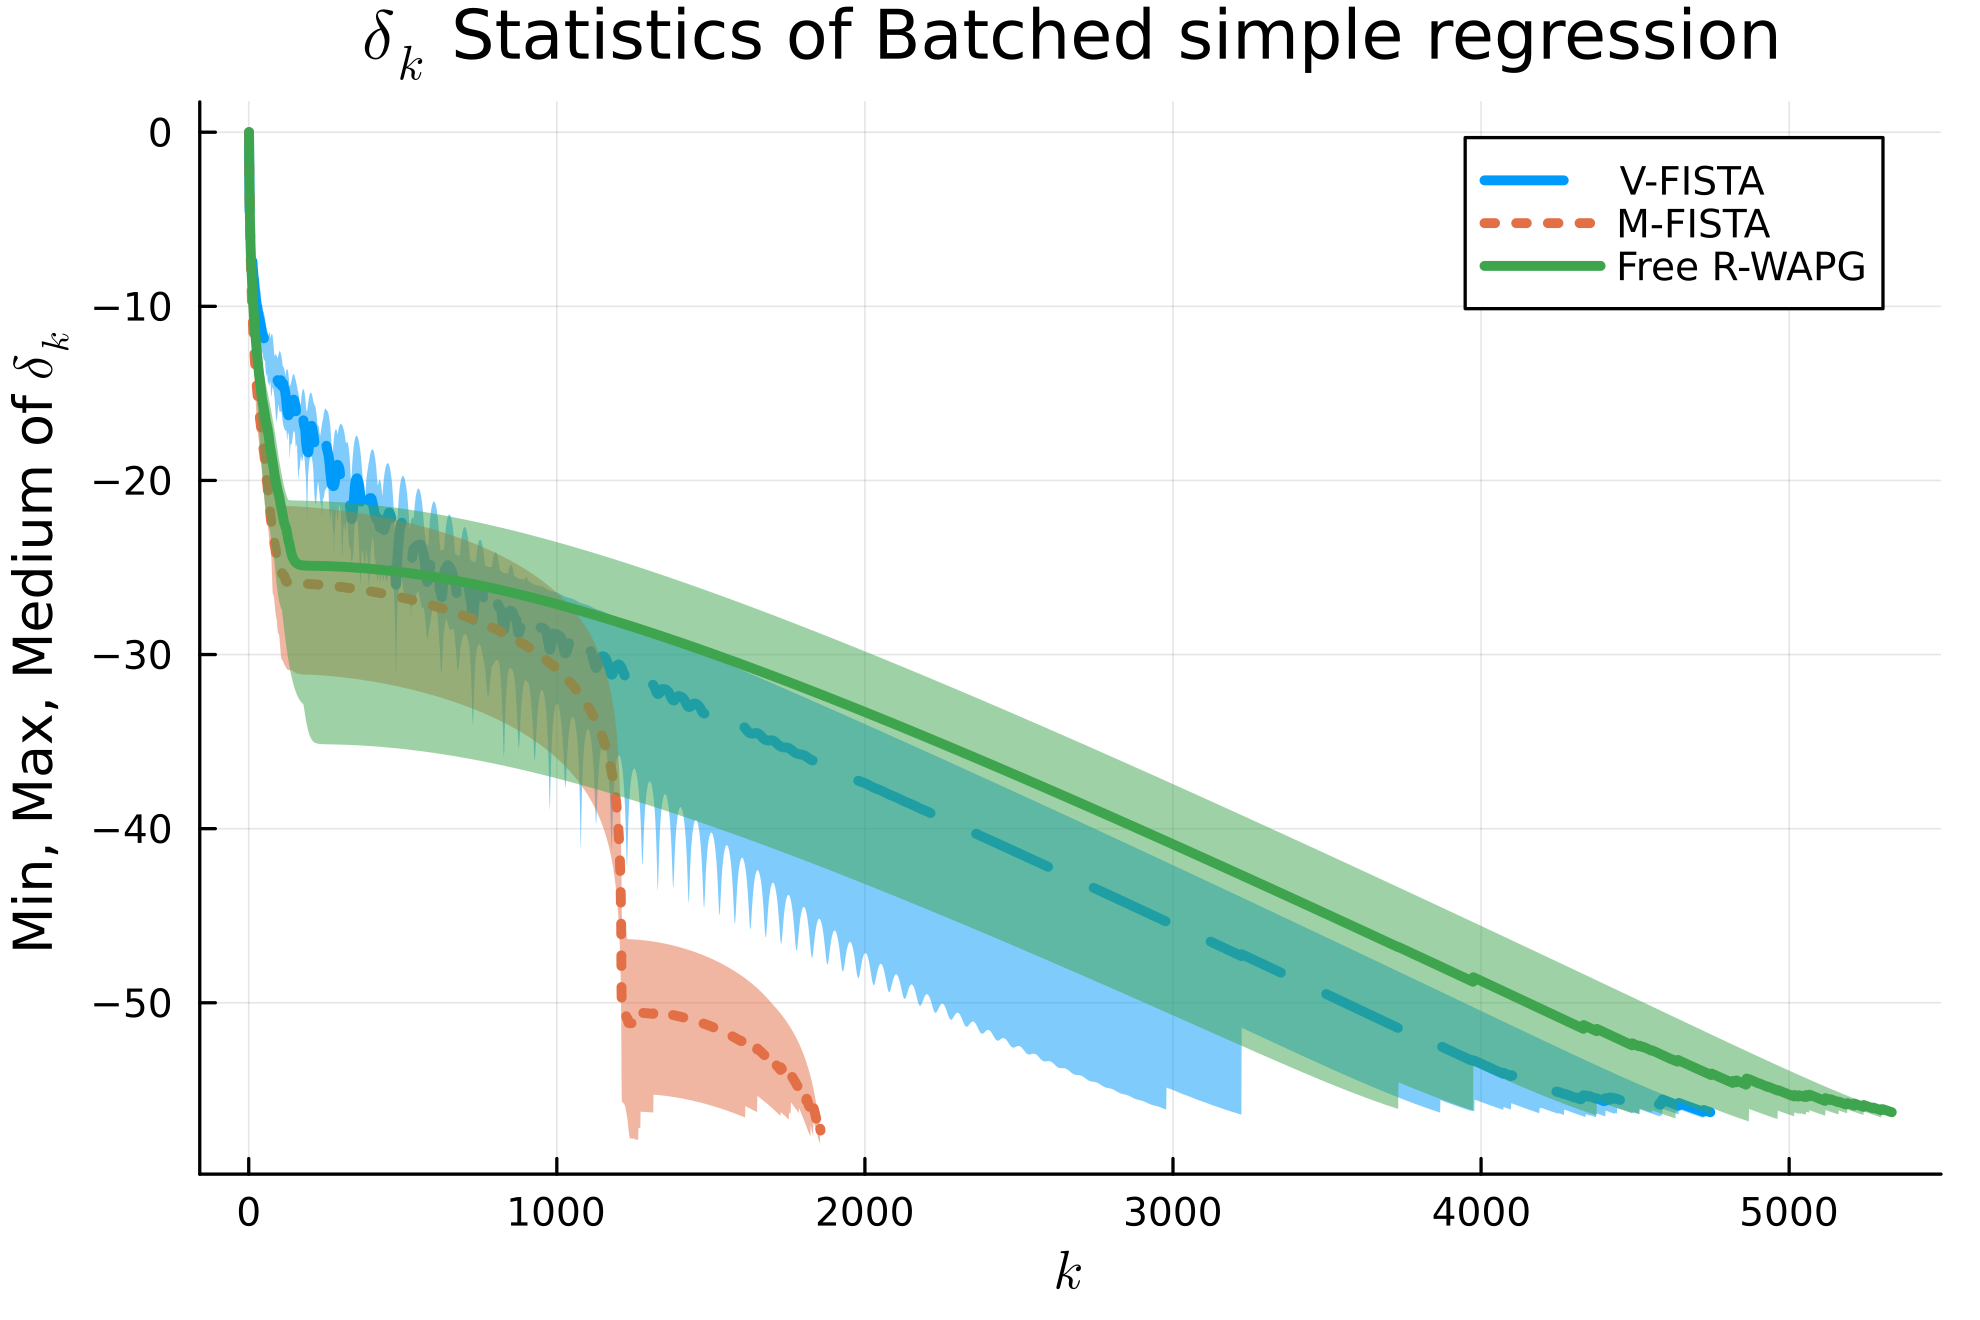
\includegraphics[width=\textwidth]{assets/simple_regression_batched-256.png}
                \caption{$N = 256$, simple convex quadratic.}
            \end{subfigure}
            \hfill
            \begin{subfigure}[b]{0.47\textwidth}
                \centering
                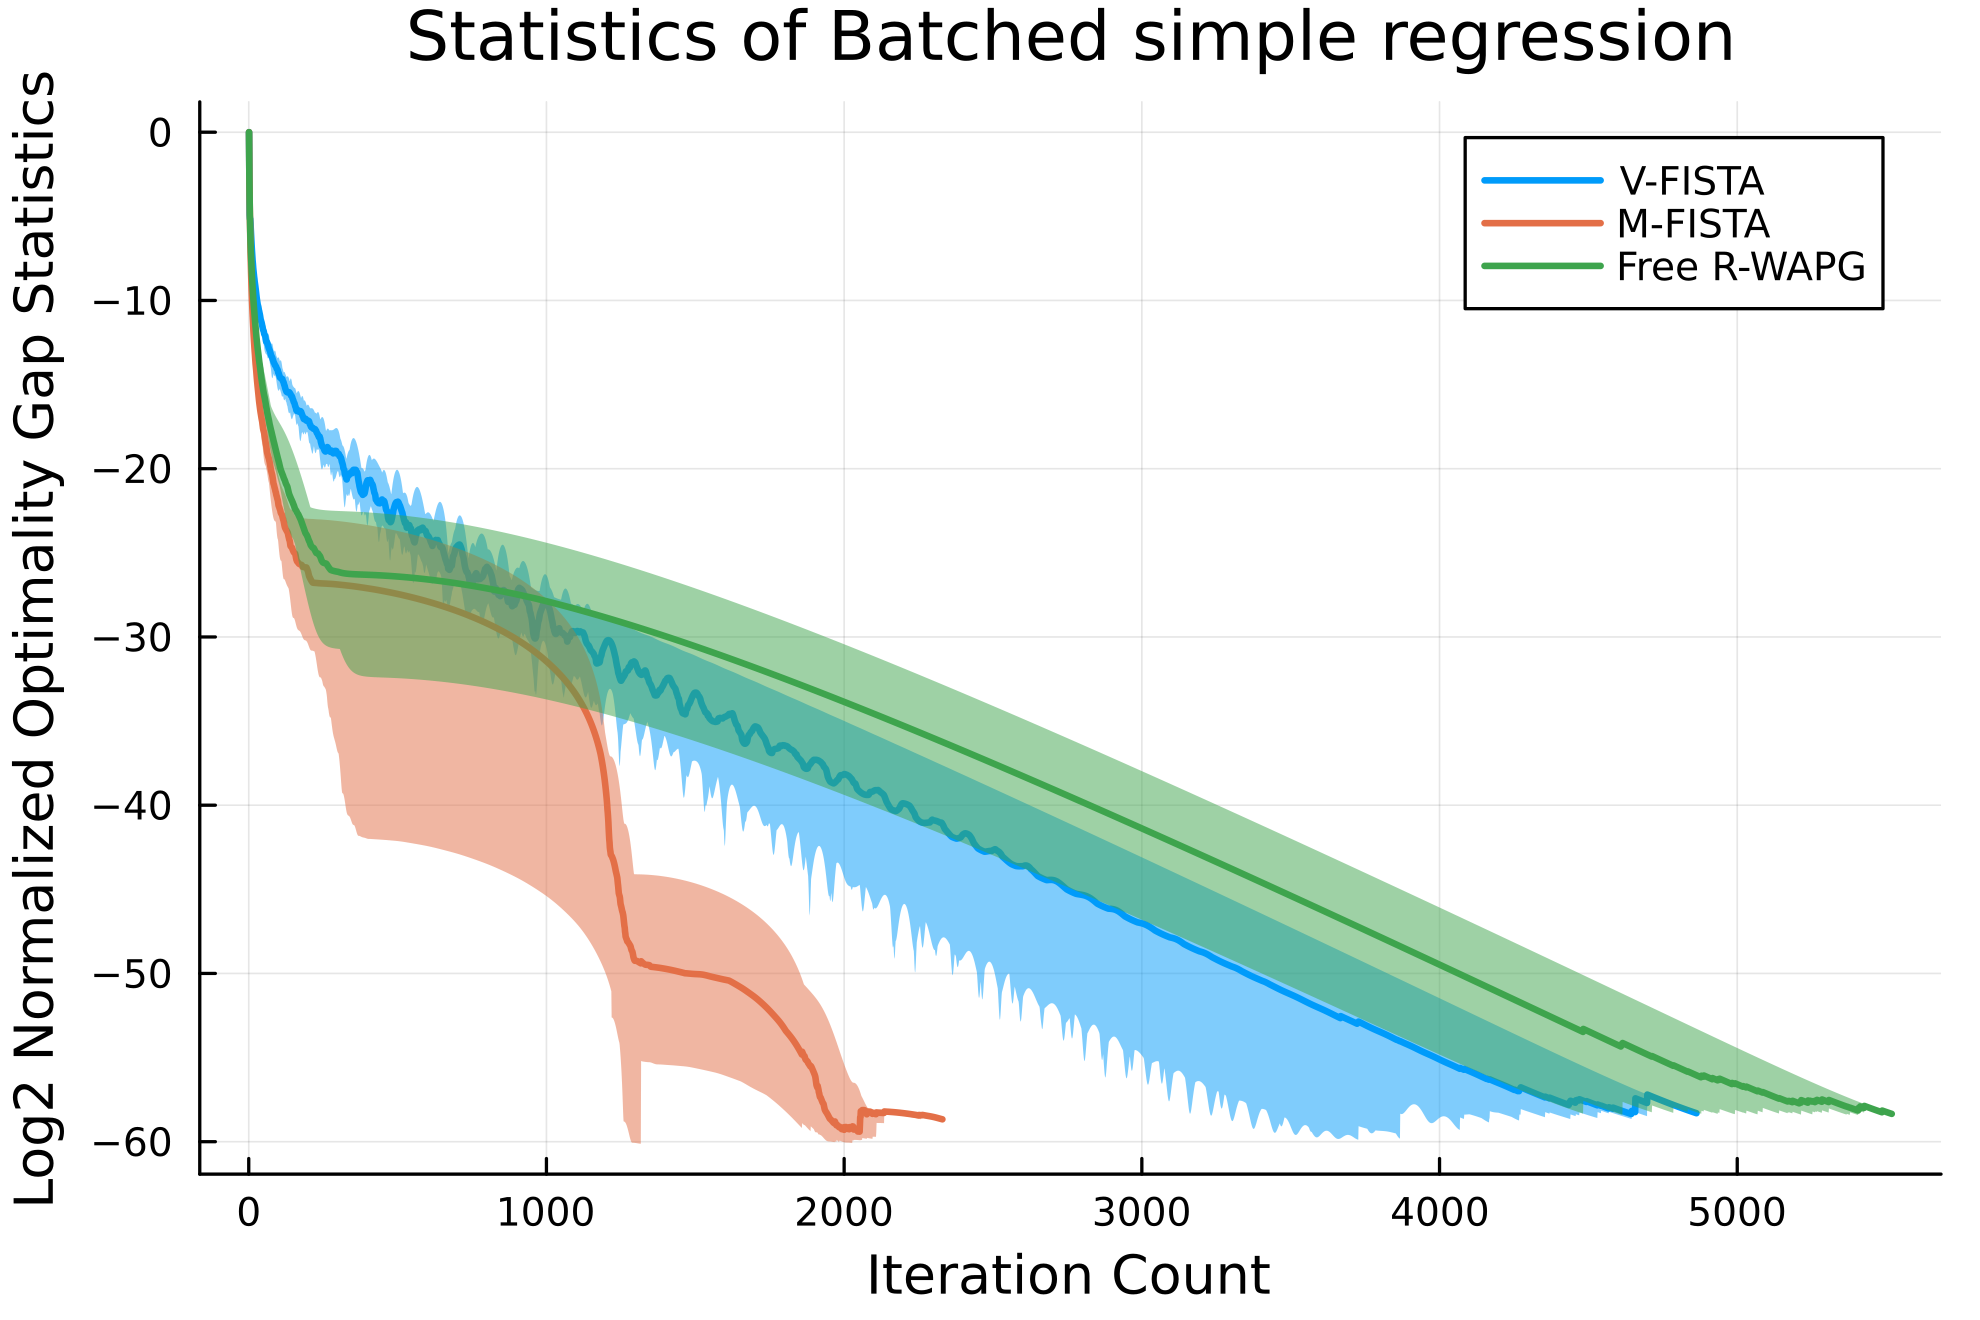
\includegraphics[width=\textwidth]{assets/simple_regression_batched-1024.png}
                \caption{$N = 1024$, simple convex quadratic. }
            \end{subfigure}
            \caption{Simple convex quadratic experiments results for V-FISTA, M-FISTA, and R-WAPG. }
            \label{fig:simple-quadratic-NOG}
        \end{figure}
        \par
        Another quantity that maybe interesting other than $\delta_k$ would be the estimated value of $\mu$ during at each iteration $k$. 
        This $\mu$ parameter should converge to the true value. 
        One individual experiment is carried out for the R-WAPG algorithm and the value of $\mu$ at each iteration is being recorded as well. 
        Figure \ref{fig:simple-quadratic-r-wapg-mu-estimates} showcases the results. 
        The values oscillate and converges to the true $\mu$ value. 
        Observe that the iteration when the estimates are nearing the true value corresponds to the iteration when the algorithm plateau away from its initial fast descent. 
        \begin{figure}[H]
            \centering
            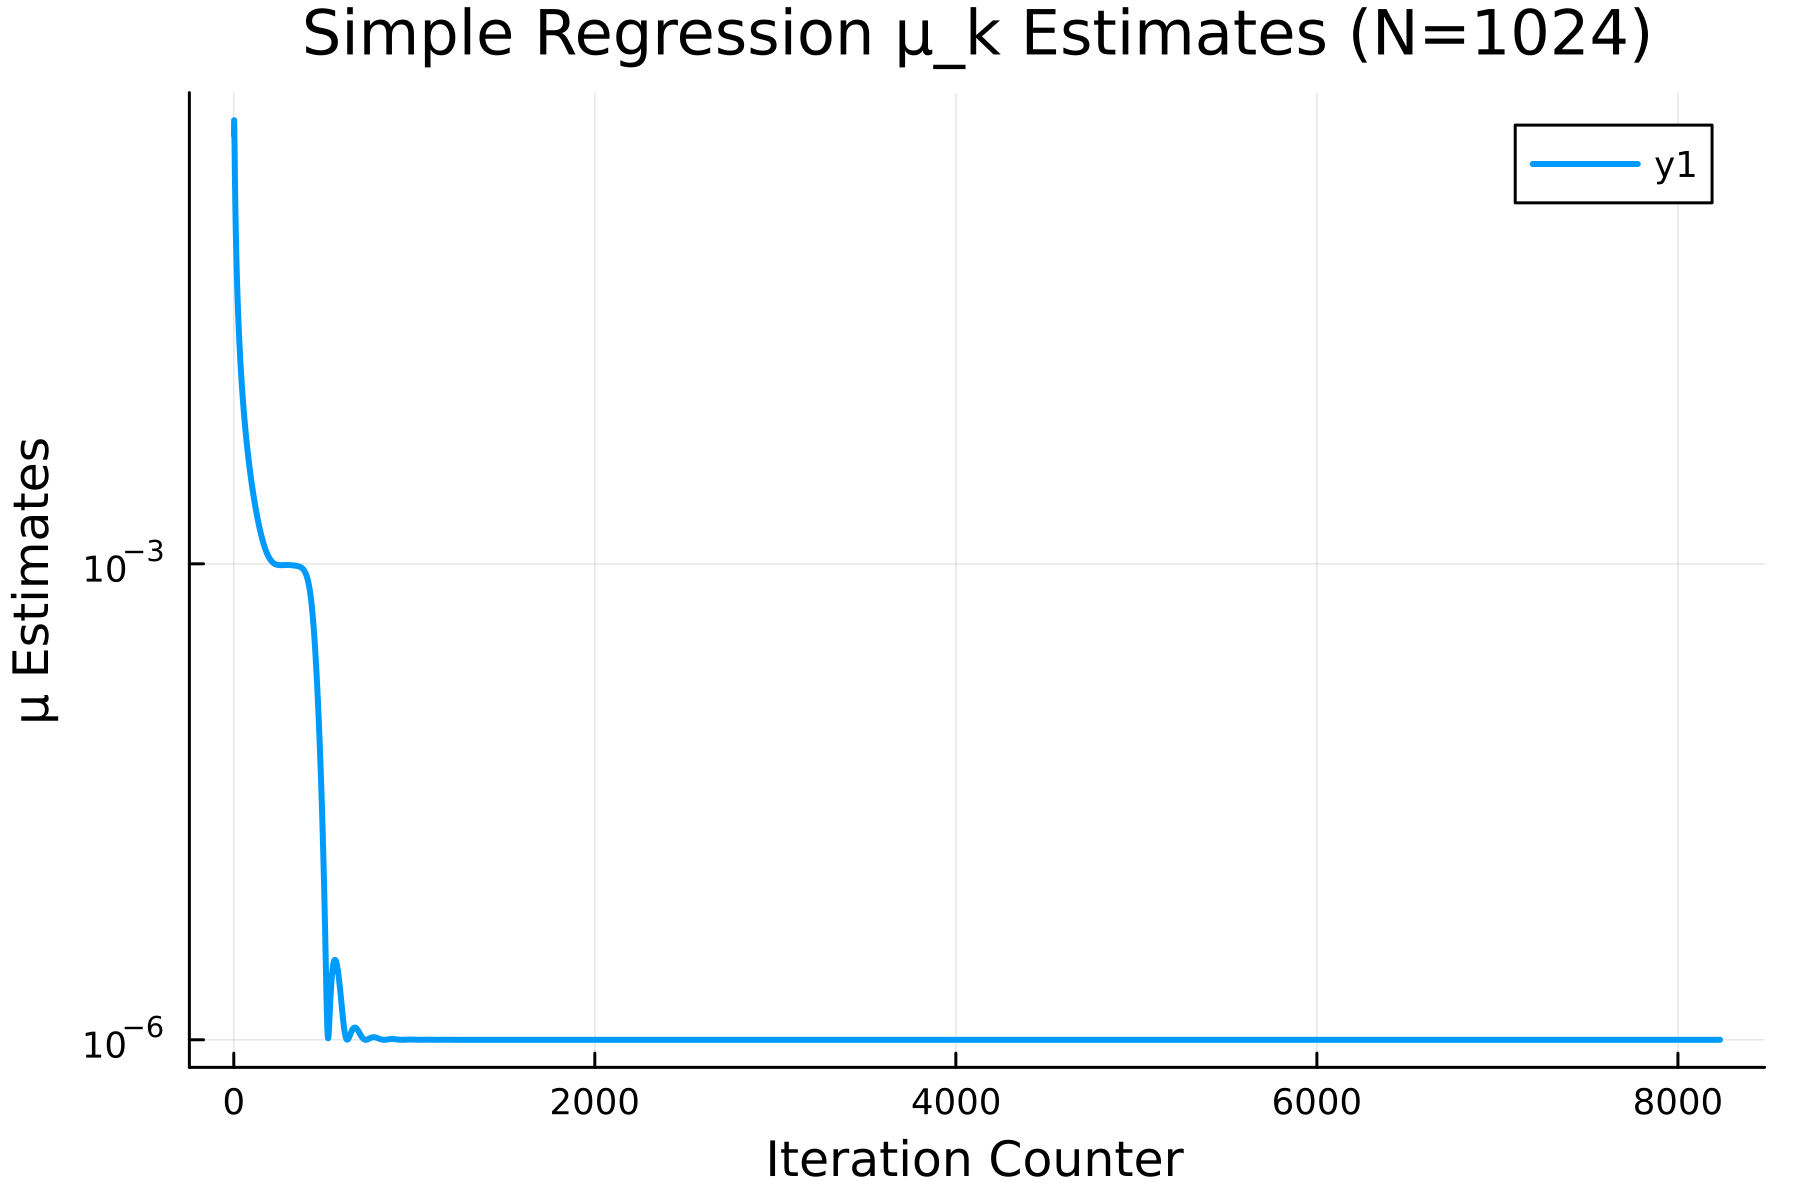
\includegraphics[width=0.64\textwidth]{assets/simple_regression_loss_sc_estimates_1024.png}
            \caption{$N = 1024$, the $\mu$ estimates produced by Algorithm \ref{alg:free-rwapg} (R-WAPG) is recorded. }
            \label{fig:simple-quadratic-r-wapg-mu-estimates}
        \end{figure}

    \subsubsection{LASSO}
        This section present results of numerical experiment for solving the (least absolute shrinkage and
        selection operator) LASSO problem proposed by 
        Tibshirani \cite{tibshirani_regression_1996}. 
        The problem of LASSO has smooth, nonsmooth additive and the problem is given by: 
        \begin{align*}
            \min_x
            \left\lbrace
                \frac{1}{2}\Vert Ax - b\Vert^2 + \lambda\Vert x\Vert_1
            \right\rbrace. 
        \end{align*}
        The smooth part is $f =\frac{1}{2}\Vert Ax - b\Vert^2$ and the nonsmooth is $g = \lambda\Vert x\Vert_1$. 
        The objective function is coercive and the exact minimum, or minimizers are unknown. 
        We perform numerical experiments using V-FISTA, M-FISTA and R-WAPG on this problem. 
        The parameters for setting up the problem now follow. 
        \begin{enumerate}
            \item $M, N$ are constants. 
            \item $A \in \RR^{M\times N}$ is a matrix of i.i.d random variable, taken from a standard normal distribution. 
            \item $L, \mu$, the Lipschitz constant and the strong convexity constant for the smooth part of the objective are not known prior, and it's estimated through $A$ by $\mu = 1/\Vert (A^TA)^{-1}\Vert$ and $L = \Vert A^TA\Vert$. 
            \item $x^+ = [1\; -1\; 1 \; \cdots ]^T \in \RR^N$, it's a vector with alternating $1, -1$ in it. 
            \item Given $x^+$, it has $b = Ax^+ \in \RR^M$. 
            \item Given $A$, estimations for $L,\mu$ are given by $L = \Vert A^TA\Vert$, $\mu = \Vert (A^TA)^{-1}\Vert^{-1}$. 
            \item $x_0\in \RR^N$ is the initial guess. Its elements are random i.i.d variable realized from the standard normal distribution. 
            \item $\epsilon > 0$ is the tolerance the controls the termination criteria for test algorithms. 
        \end{enumerate}
        Experiments were conducted using V-FISTA, M-FISTA and R-WAPG with $(M, N) = (64, 256)$ and $(M, N) = (64, 128)$. 
        Matrix $A$ is fixed and the for all test algorithms and all repetitions. 
        The same experiment are repeated 30 times, but each time, we fix a different random initial condition $x_k$ for all test algorithms. 
        The aggregate statistics of $\delta_k$ are collected for all repetitions, and then grouped by the respective algorithm. 
        The results are showcased in Figure \ref{fig:batched-lasso}. 
        The bump on the curve is due to a subset of test instances of the 30 repetition where the algorithms take larger number of iterations to terminate. 
        \begin{figure}[H]
            \begin{subfigure}[b]{0.47\textwidth}
                \centering
                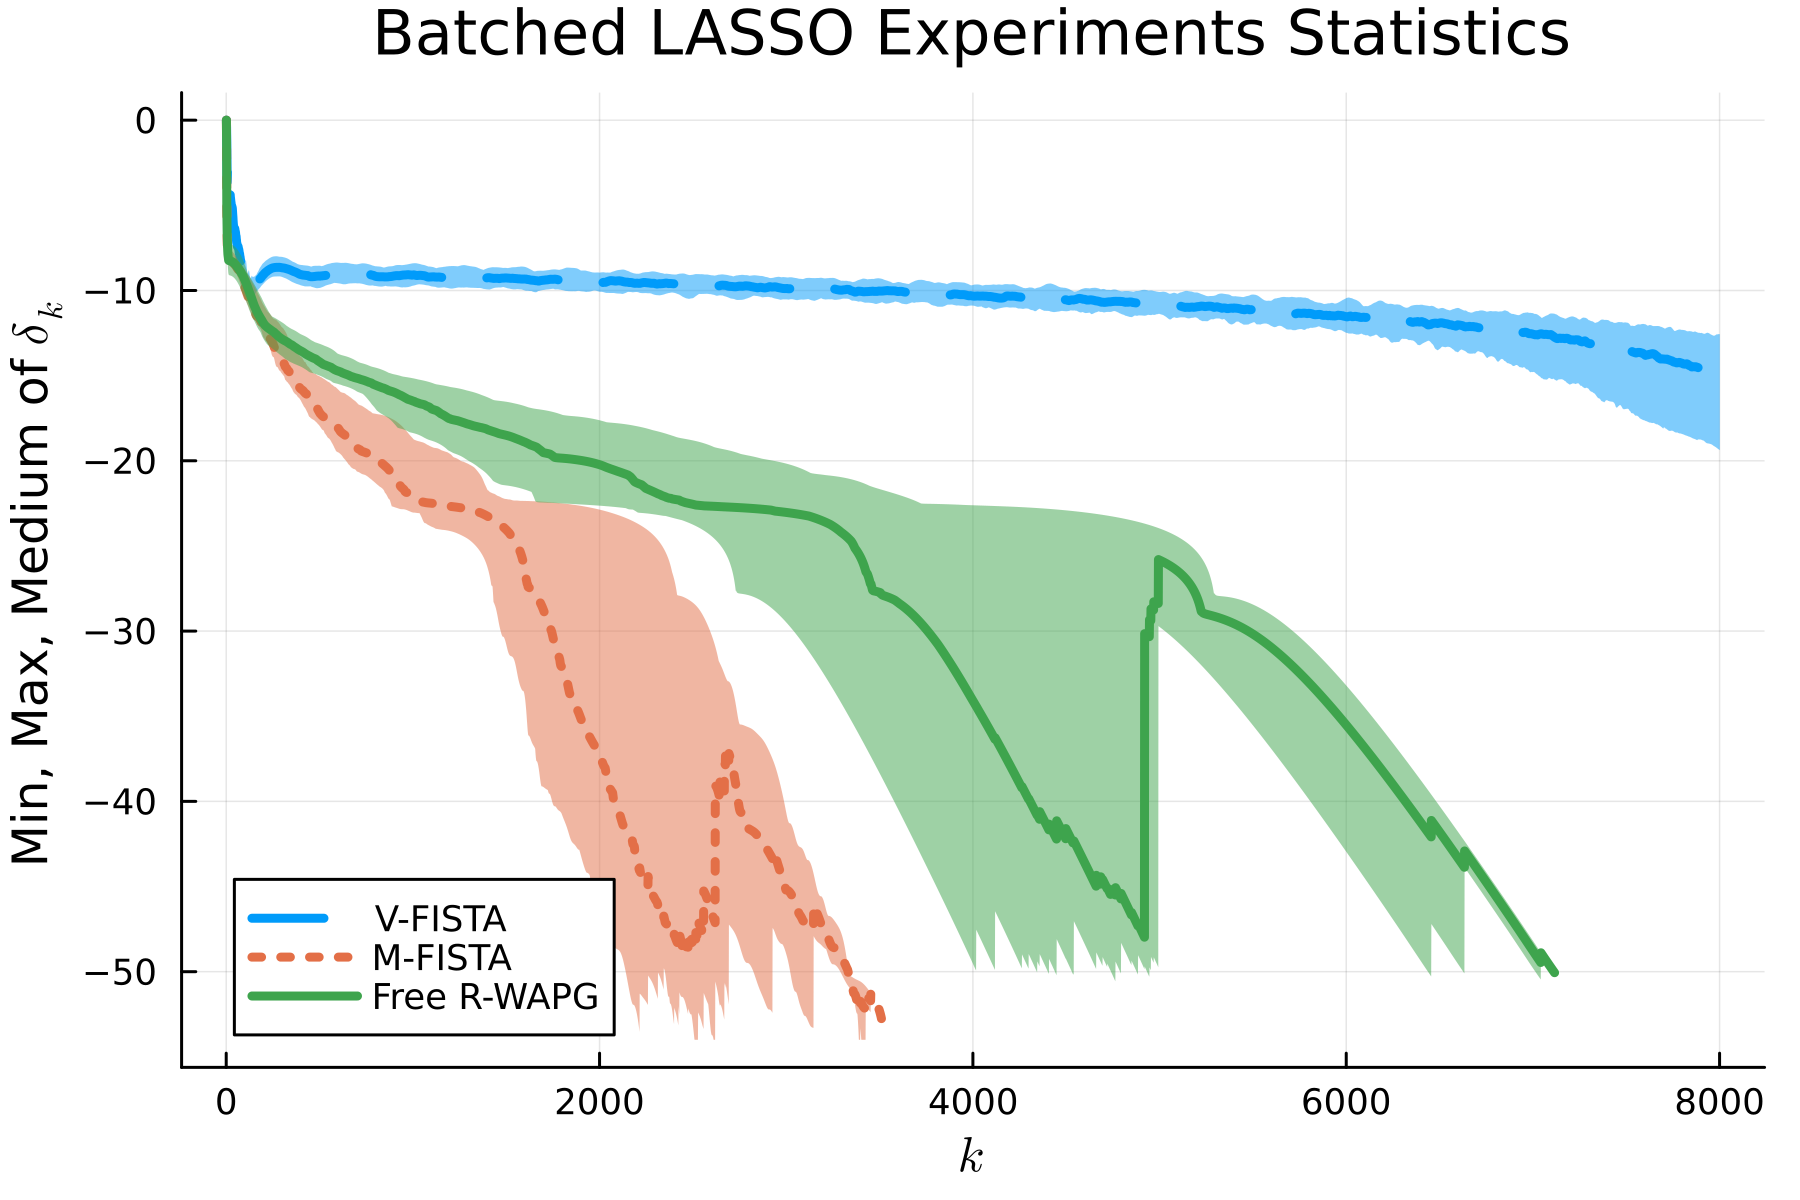
\includegraphics[width=\textwidth]{assets/lasso_batched_statistics_64-256.png}
                \caption{LASSO experiment with $M = 64, N = 256$. Plots of minimum, maximum, and median $\delta_k$ with estimated $F^*$. }
            \end{subfigure}
            \hfill
            \begin{subfigure}[b]{0.47\textwidth}
                \centering
                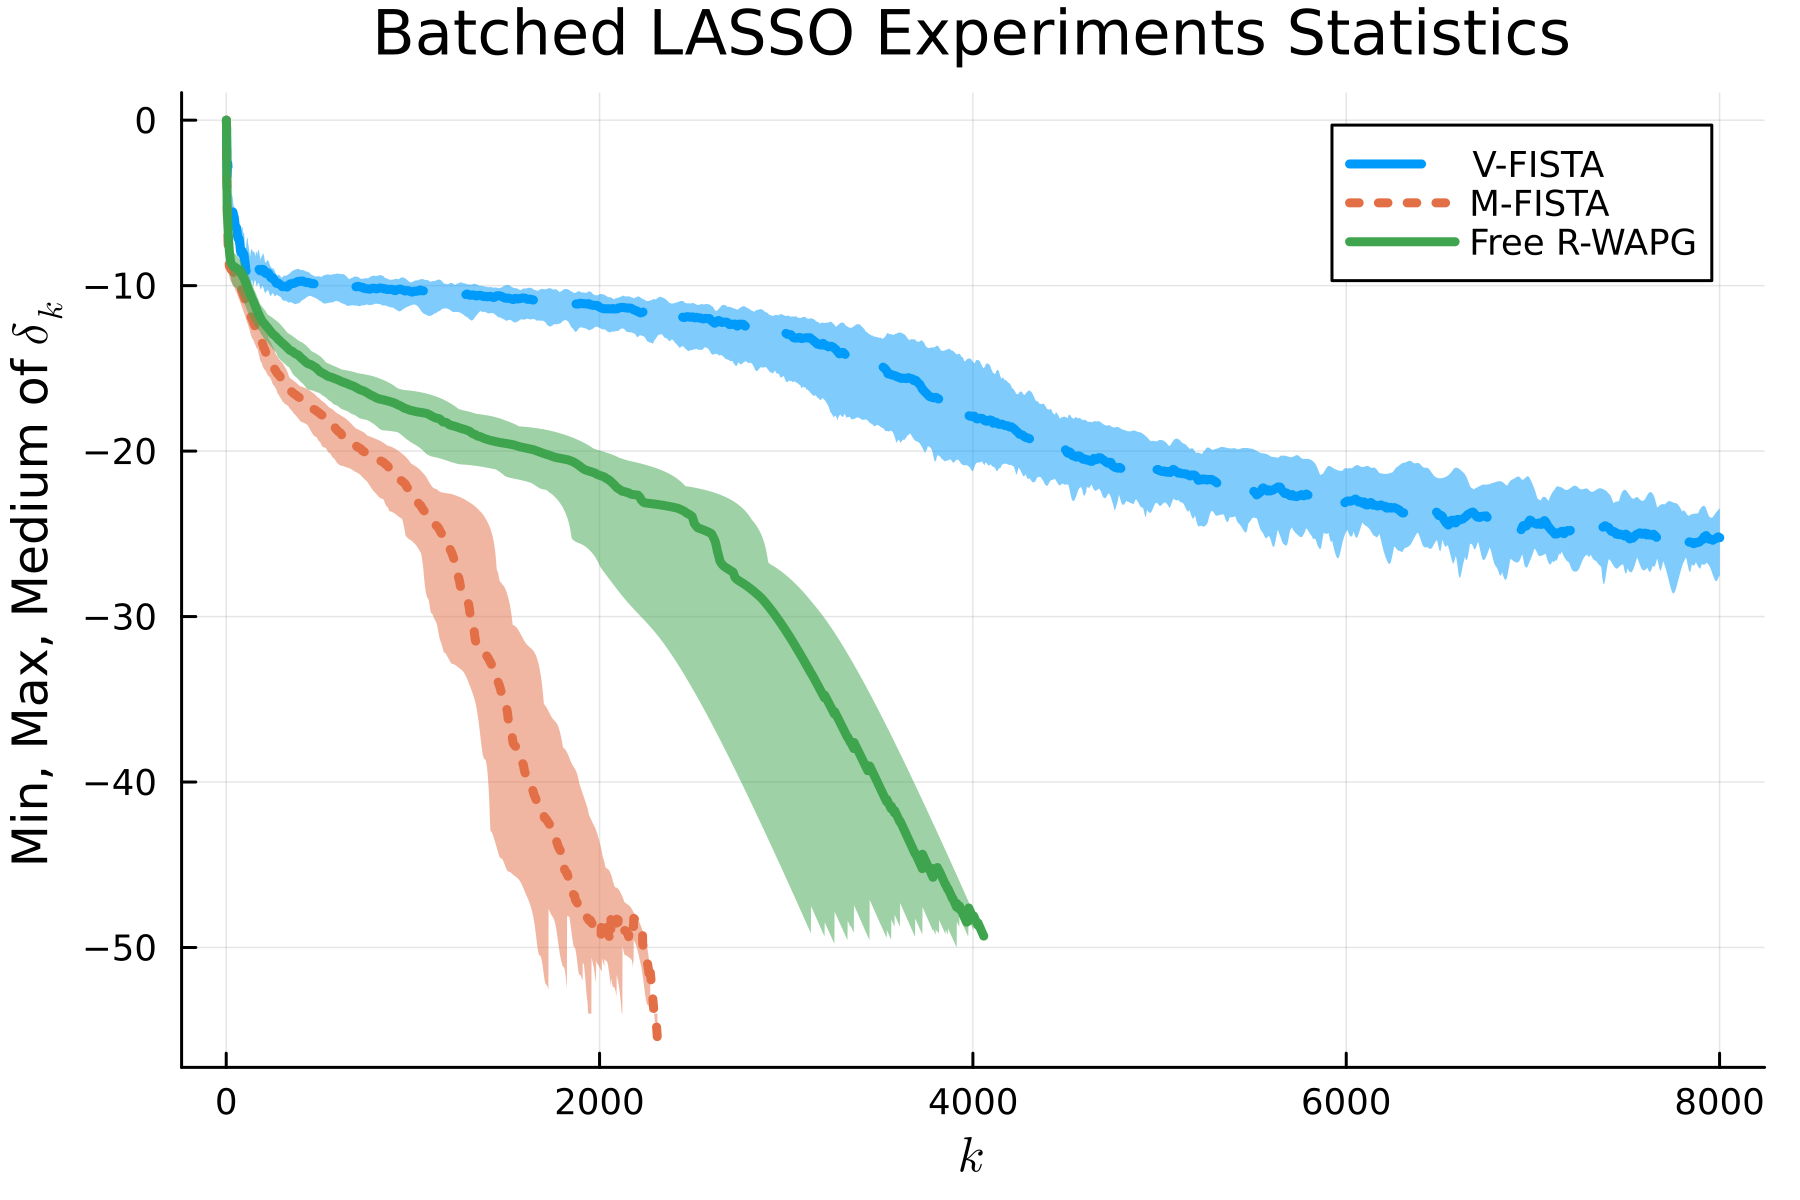
\includegraphics[width=\textwidth]{assets/lasso_batched_statistics_64-128.png}
                \caption{LASSO experiment with $M = 64, N = 128$. Plots of minimum, maximum, and median $\delta_k$ with estimated $F^*$. }
            \end{subfigure}
            \caption{LASSO experiments. }
            \label{fig:batched-lasso}
        \end{figure}
        \par
        Another quantity of interest is the estimates of $\mu$ on each iteration of the algorithm. 
        A single experiment were conducted and the estimates and $\delta_k$ are showcased in Figure \ref{fig:single-lass-mu-estimates}
        \begin{figure}[H]
            \begin{subfigure}[b]{0.47\textwidth}
                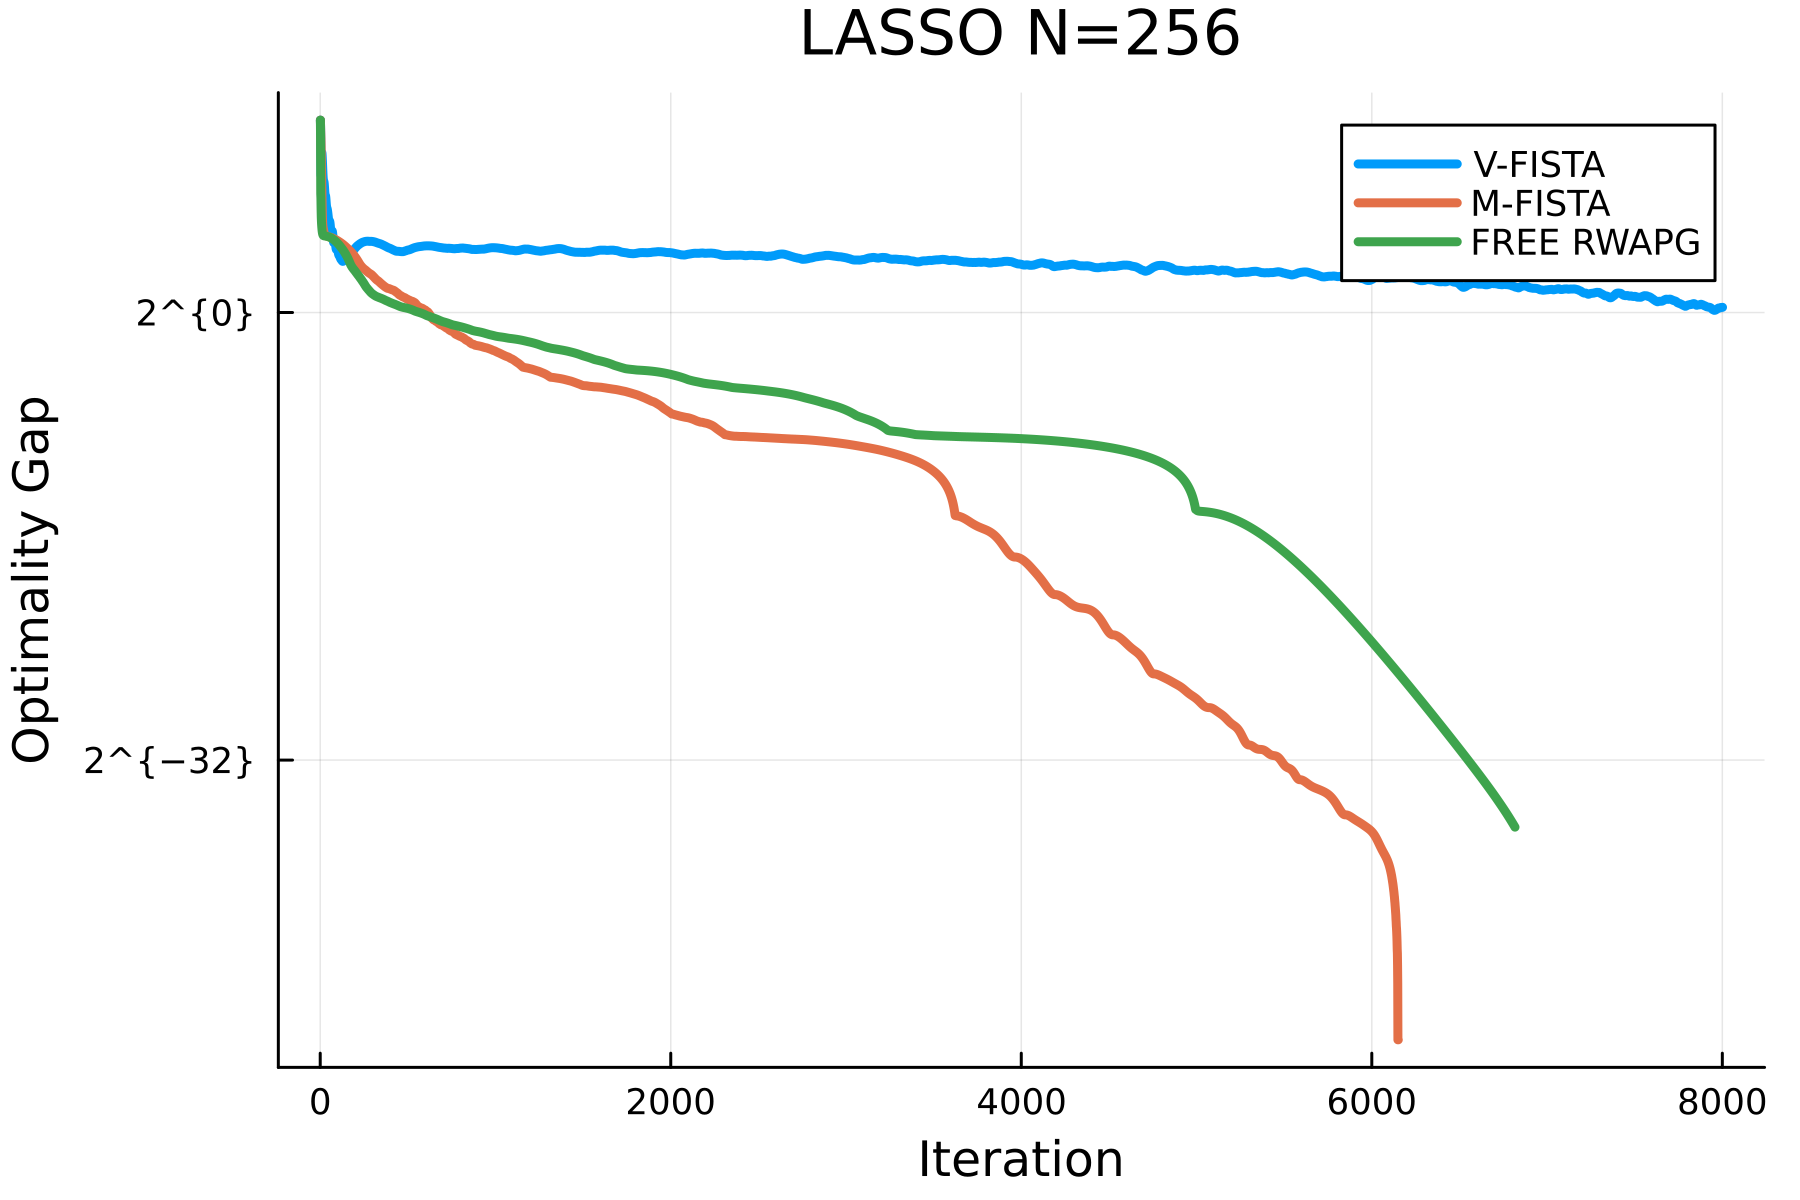
\includegraphics[width=\textwidth]{assets/lasso_loss_256.png}
                \caption{Single lasso experiment plot of $\delta_k$ with.  }
            \end{subfigure}
            \hfill
            \begin{subfigure}[b]{0.47\textwidth}
                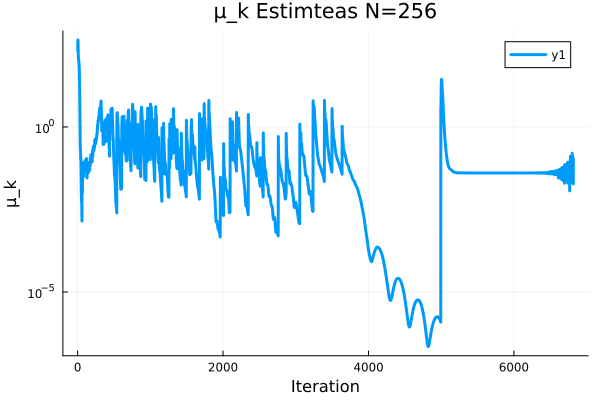
\includegraphics[width=\textwidth]{assets/lasso_sc_estimates_256.png}
                \caption{The $\mu$ estimated by test algorithms for one LASSO experiment. }
            \end{subfigure}
            \caption{A single LASSO experiment results, with $M = 64, 256$. }
            \label{fig:single-lass-mu-estimates}
        \end{figure}
        For this specific experiment showed in the figure, the estimated value of $\mu, L$ which we feed into V-FISTA are $\mu = 7.432363627613958\times 10^{-18}$ and $L = 2321.737206983643$. 
        One of the most important feature is that the estimate $\mu$ doesn't converge to the true value, but it didn't affect the convergence of $\delta_k$. 

    \subsection{Future works for R-WAPG}
        The R-WAPG framework neglected a detail in the literatures. 
        Our future works would extend the frameworks and include this detail. 
        \subsubsection{Nesterov's idea of strong convexity transfer}
            We consider the case that $F = f + g$ where, $f$ is $L$ Lipschitz smooth, $\mu_f \ge 0$ strongly convex and $g$ is closed convex. 
            In Nesterov's 2013 paper \cite{nesterov_gradient_2013}, he considers accelerated  minimization problem $\phi = f + \Psi$ with $f$ $L_f$ smooth and $\Psi$ being $\mu_\Psi \ge 0$ strongly convex. 
            \par
            This detail on itself is not necessarily interesting, since without lost of generality, we can always do the splitting $f + \mu_\Psi/2 \Vert \cdot\Vert^2$ and $\Psi - \mu_\Psi/2\Vert \cdot\Vert^2$ instead so that the smooth part is $\mu_\Psi \ge 0$ strongly convex. 
            It's an interesting detail we should consider because: 
            \begin{enumerate}
                \item A strongly convex nonsmooth parts still gives linear convergence by Theorem 6 in Nesterov's 2013 \cite{nesterov_gradient_2013}. 
                \item The strong convexity constant can be easily estimated via a routine specified as (5.14) in Nesterov 2013 \cite{nesterov_gradient_2013} and the complexity of the estimation is bounded precisely. 
            \end{enumerate}
            (i) indicates that our theories of R-WAPG is incomplete, since it doesn't predict linear convergence when $g$ is strongly convex. 
            (ii) indicates that splitting the strongly convex objective so that it's with the proximal operator gives computational advantage. 
            \par
            Furthermore, Nesterov was not the only person who thought about it.
            In 
            Chambolle, Pock \cite{chambolle_introduction_2016} Algorithm 5, several variants of the FISTA algorithm were captured together into one formulation, and it assumes that $F = f + g$ where $f, g$ has strong convexity index $\mu_f \ge 0, \mu_g \ge 0$, and $F$ is $\mu := \mu_f + \mu_g \ge 0$ strongly convex. 
            
        % \subsubsection{Tying up some loose ends}
        %     \todoinline{\noindent
        %         In terms of practice, we are missing convergence rate of Free-RWAPG, and the convergence of the norm of the gradient method for R-WAPG. 
        %     }

\section{Catalyst accelerations and future works}\label{sec:catalyst}
    We start by introducing important assumptions and notations for the Catalyst Meta Acceleration Frameworks. 
    \begin{assumption}\label{ass:catalyst1}
        Given any $\beta > 0$ and $y \in \RR^n$, and $F: \RR^n\rightarrow \overline \RR$ is $\mu \ge 0$ strongly convex and closed. 
        Assume that minimizer exists for $F$ and the minimum is $F^*$. 
        For all $x,y\in \RR^n, \beta > 0$ define the model function: 
        \begin{align*}
            \mathcal M^{\beta^{-1}}_F(x; y) &:= 
            F(x) + \frac{\beta}{2}\Vert x - y\Vert^2.
        \end{align*}
        We define the Moreau Envelope at $y \in \RR^n$ to be $\mathcal M^*_{F,\beta^{-1}}(y) := \min_{x\in \RR^n} \mathcal M_F^{\beta^{-1}}(x; y)$. 
        We denote $\mathcal J_{\beta^{-1}F}$ to be the resolvent operator for subgradient of $F$, which is also called the proximal operator. 
    \end{assumption}
    \begin{definition}[Absolute termination criterion C1]\label{def:catalyst-termination-c1}
        Take $F$ as given by Assumption \ref{ass:catalyst1}.
        For $\epsilon > 0, \kappa > 0$ and $x \in \RR^n$, the absolute criterion C1 characterizes the set of inexact proximal iterates by: 
        \begin{align*}
            \mathcal J_{\kappa^{-1} F}^\epsilon (x) := 
            \left\lbrace
                y \in \RR^n \left | \; 
                        \mathcal M^{1/\kappa}_F (y; x) - 
                        \mathcal M^*_{F, 1/\kappa}(x) \le \epsilon
                \right.
            \right\rbrace. 
        \end{align*}
    \end{definition}
    \begin{remark}
        Setting $\epsilon = 0$, we have the exact definition of the exact resolvent given as $\mathcal J_{\beta^{-1}}y = \mathcal J^0_{\beta^{-1}}y$. 
    \end{remark}
    \textbf{Organizations now follow}. 
    Section \ref{ssec:catalyst-intro} gives the main ideas behind the Catalyst Acceleration Framework. 
    It follows Lin et al.'s first paper \cite{lin_universal_2015} on Catalyst Acceleration and summarizes the convergence analysis of the algorithm. 
    Section \ref{ssec:catalyst-second-paper} introduces Lin et al.'s second paper \cite{lin_catalyst_2018} on Catalyst which considers the improved relative error condition stated in Definition \ref{def:catalyst-termination-c2} and discusses its significance. 
    This condition improves the overall complexity and inspired nonconvex gradient based 4WD Catalyst by Paquette \cite{paquette_catalyst_2018}. 
    
    \subsection{Introduction to Catalyst}\label{ssec:catalyst-intro}
        Inspired by accelerated proximal point Method (APPM) from Güler \cite{guler_new_1992}, and Inexact Proximal Point Method (IPPM) of Rockafellar 1976 \cite{rockafellar_monotone_1976}, Lin \cite{lin_universal_2015} proposed a generic method taking inspirations from the convergence claims   of (APPM) to accelerate Variance Reduced Method (VRM). 
        The fact that VRMs are incremental method that is not slower than full gradient descent in complexity is most relevant to our discussion. 
        See Gower's guide \cite{gower_variance-reduced_2020} for more information on variance reduced methods in machine learning. 
        \par
        In brief, VRM is a type of incremental methods for solving a large sum problem: $F(x) = \sum_{i = 1}^{N} f_i(x)$ in machine learning.
        See Bertsekas's surveys \cite{bertsekas_incremental_2011,bertsekas_incremental_2017} for more context. 
        VRM can be deterministic, or stochastic. 
        When it's stochastic, the theories focus on the expected optimality gap: $\mathbb E[F(x_k) - F^*]$. 
        Let's assume for simplicity of discussion that it's deterministic, so we focus on: $F(x_k) - F^*$. 
        \par 
        VRM stabilizes the estimate of gradient using information from all or a subset of gradients evaluated at previous iterates. 
        In each iteration, it accesses the gradient of a few samples are used to attain a new estimate of the gradient with minimum additional calculations.  
        This gives better complexity than full gradient descent over all. 
        Compare to traditional stochastic gradient, VRM produces smaller variance of the estimated gradient near the minimizer which gives faster convergence rate. 
        Major examples of VRMs include SVRG by Xiao, Zhang \cite{xiao_proximal_2014}, Finito by Defazio et al. \cite{defazio_finito_2014}, SAG by Schmidt et al. \cite{schmidt_minimizing_2017}, and SAGA by \cite{defazio_saga_2014}. 
        \par
        Next, we introduce the first Catalyst algorithm in \cite{lin_universal_2015}. 
        \begin{definition}[Lin's Universal Catalyst Acceleration]\label{def:lin-catalyst-original}\; \\
            Let $F:\RR \rightarrow \overline \RR$ be $\mu \ge 0$ strongly convex and closed. 
            Let the initial estimate be $x_0 \in \RR^n$, fix parameters $\kappa > 0$ and $\alpha_0 \in (0, 1]$. 
            Let $(\epsilon_k)_{k \ge 0}$ be an absolute error sequence chosen for the evaluation for inexact proximal point method. 
            \begin{tcolorbox}
                Initialize $x_0 = y_0$. Then the algorithm generates $(x_k, y_k)_{k\ge 0}$ for all $k \ge 1$ such that: 
                \begin{align*}
                    & \text{find } x_k \in \mathcal J_{\kappa^{-1}F}^{\epsilon_k} y_{k - 1}, 
                    \\
                    & \text{find } \alpha_k \in (0, 1) \text{ such that } \alpha_k^2 = (1 - \alpha_k)\alpha_{k - 1}^2 + (\mu/(\mu + \kappa))\alpha_k,
                    \\
                    & 
                    y_{k} = x_k + \frac{\alpha_{k - 1}(1 - \alpha_{k - 1})}{\alpha_{k - 1}^2 + \alpha_k}(x_k - x_{k - 1}). 
                \end{align*}
            \end{tcolorbox}
        \end{definition}
        \begin{remark}
            The above algorithm is Algorithm 1 from the first paper on Catalyst Acceleration by Lin et al. \cite{lin_universal_2015}. 
            The explicit formula for $\alpha_k$ is the larger root of solving the quadratic equation given by: 
            \begin{align*}
                \alpha_k &= 
                \frac{1}{2}\left(
                    q - \alpha_{k - 1}^2 + \sqrt{(q + \alpha_{k - 1})^2 + 4 \alpha_{k - 1}}
                \right), 
            \end{align*}
            where $q = \mu/(k + \mu)$. 
            The choices for $\kappa, \epsilon_k$ will come later. 
        \end{remark}
        \textbf{Notations now follows}. 
        With a fixed regularization parameter $\kappa > 0$, the outer loop (i.e: Definition \ref{def:lin-catalyst-original}) produces $(y_{k}, x_k)_{k \ge k}$ denote it by $\mathbb A$. 
        Typically, an iterative scheme (i.e: VRM) with a known complexity is assigned to find inexact proximal iterates $x_k \in {\mathcal J}_{\kappa^{-1}F}^{\epsilon_k} (y_{k - 1})$. 
        We refer to it as the inner loop and denote it by $\mathbb M$. 
        Without loss of generality assume it generates some iterates $(z_{k, t})_{t \ge 0}$ where $k$ is the corresponding iteration counter of the outer loop and $t$ is the iteration counter of the inner loop. 
        \par 
        The choice of absolute error sequence $(\epsilon_k)_{k \ge 0}$ determines the iteration complexity of both $\mathbb A, \mathbb M$. 
        The total iteration complexity of Catalyst counts the total number of inner loop iteration given  the number of outer loop iterations. 
        The term ``iteration complexity'' refers to the number of iterations required to achieve a desired accuracy, a concept related to the convergence rate of the algorithm. 
        We adopt iteration complexity in the sections that follow. 
        % The term ``complexity'' refers to the total number of oracle calls, in our context it depends on the specific implementation of $\mathbb M$. 
        Since $F$ is convex, we focus on the convergence rate of the optimality gap $F(x_k) - F^*\*$ for $\mathbb A$ and convergence of the model function $\mathcal M_F^{\kappa^{-1}}(\cdot, y_{k - 1})$ for $\mathbb M$ given $y_{k - 1}, \epsilon_k$ and initial guess $z_{k, 0}$. 
        \par
        \subsubsection{Outer loop iteration complexity}
            The error sequence $(\epsilon_k)_{k \ge 0}$ controls the convergence rate of $F(x_k) - F^*$ of the outer loop $\mathbb A$. 
            Depending on either $\mu > 0$, or $\mu = 0$, the choice of $(\epsilon_k)_{k\ge 0}$ differs. 
            The theorems that follow state the error sequence required for the outer loop to retain optimal convergence rate, they are Theorem 3.3, 3.1 in Lin et al. \cite{lin_universal_2015}. 
            \begin{theorem}[Outer loop convergence strongly convex]\label{thm:err-seq-outer-s-cnvx}
                For $\mathbb A$ with regularization parameter $\kappa > 0$. 
                Assume that $F$ is $\mu > 0$ strongly convex. 
                Choose $\alpha_0 = \sqrt{q}$ with $q = \mu/(\kappa + \mu)$ and the error sequence 
                $$
                \begin{aligned}
                    \epsilon_k = \frac{2}{9}(F(x_0) - F^*)(1 - \rho)^k \quad \text{with }\quad 
                    \rho < \sqrt{q}. 
                \end{aligned}
                $$
                Then the $\mathbb A$ generates $(x_{k})_{k \ge 0}$ such that 
                $$
                \begin{aligned}
                    F(x_k) - F^* &\le 
                    C(1 - \rho)^{k + 1} (F(x_0) - F^*) \quad \text{ with }\quad 
                    C = \frac{8}{(\sqrt{q} - \rho)^2}. 
                \end{aligned}
                $$
            \end{theorem}
            \begin{remark}
                Suggested by Lin et al., $\rho$ is at the discretion of the practitioner, take for example $\rho = 0.9\sqrt{q}$ would work. 
            \end{remark}
            \begin{theorem}[Outer loop convergence convex but not strongly convex]\label{thm:erro-seq-outer-cnvx}\;\\
                For $\mathbb A$ with regularization parameter $\kappa > 0$. 
                Assume that $F$ is convex but with strong convexity constant $\mu = 0$. 
                Choose $\alpha_0 = (\sqrt{5} - 1)/2$ and the error sequence 
                \begin{align*}
                    \epsilon_k &= \frac{2(F(x_0) - F^*)}{9(k + 2)^{4 + \eta}} \quad 
                    \text{with}\quad \eta > 0. 
                \end{align*}
                Take $x^*$ to be a minimizer of $F$. 
                Then algorithm $\mathbb A$ generates $(x_k)_{k \ge0}$ such that it has a convergence rate of 
                \begin{align*}
                    F(x_k) - F^* &\le 
                    \frac{8}{(k + 2)^2}\left(
                        \left(1 + \frac{2}{\eta}\right)^2(F(x_k) - F^*)
                        + \frac{\kappa}{2}\Vert x_0 - x^*\Vert^2
                    \right).
                \end{align*}
            \end{theorem}
            \begin{remark}
                Suggested by Lin et al., $\eta > 0$ is at the discretion of the practitioners, for an example, $\eta = 0.1$ would work. 
            \end{remark}
            The same convergence claims hold if smaller value of $\epsilon_k$ is taken, Theorem \ref{thm:err-seq-outer-s-cnvx}, \ref{thm:erro-seq-outer-cnvx} gives the largest possible absolute error sequence $(\epsilon_k)_{k \ge 0}$ such that the convergence claim holds. 
            Of course, the results still hold if we take smaller values of $(\epsilon_k)_{k \ge0}$ as suggested by the above theorems, but it will increase the iteration complexity of $\mathbb M$. 
            \par
            Observe the absolute error sequence $(\epsilon_k)_{k \ge 0}$ requires prior knowledge of $F^*$. 
            It's poses no theoretical concerns, but it's of upmost practical concern since $F^*$ may not be accessible in practice prior to executing the algorithm. 
            In the work by Lin et al. \cite{lin_universal_2015}, the example algorithm given is in appendix item D.3 called Accelerated MISO Prox.
            It automatically builds a lower bound estimates on $F^*$ in the outer loop as the algorithm executes.
            \par 
            An inexact version of the proximal gradient inequality (similar to Theorem \ref{thm:prox-grad-ineq}) stated as Lemma A.7 in \cite{lin_universal_2015} derives the convergence of $\mathbb A$. 
            It is instrumental for formulating an inexact variant of the estimating sequence $\phi_k^* \ge F(x_k) + \xi_k$. 
            The convergence proof (outer and inner loop together) from Lin was inspired by Schmidt's Inexact Proximal Gradient method \cite{schmidt_convergence_2011}. 
            The technique of estimating sequence introduced back in Definition \ref{def:nes-est-seq} did the heavy lifting, but it results in depressingly long proof making it unsuitable for exposition here. 
            Significant pieces of theoretical innovations using Nesterov's estimating sequence are covered in details in our most recent Fall Winter 2024 MATH 590 report. 
            The parts that come will complement the report to focus on the big picture of Catalyst Acceleration. 

        \subsubsection{Inner loop complexity}
            The iteration complexity of $\mathbb M$ relates to the outer loop when warm start is used. 
            The Catalyst Paper \cite{lin_universal_2015} suggested the use of $z_{k, 0} = x_{k - 1}$ as the warm start condition. 
            With Assumption \ref{ass:linear-convergence-inner-loop}, and the suggested warm start condition,  Lin et al. derived the upper bound of the iteration complexity of $\mathbb M$.
            These results are stated as Proposition 3.2, 3.3 of their text.
            Here, \ref{prop:inner-loop-complexity-cnvx}, \ref{prop:inner-loop-complexity-s-cnvx} restates them in our notations. 
            These two theorems relate the convergence of $\mathbb M, \mathbb A$ and gives a convergence rate of $F(x_k) - F^*$ expressed using the total number of iteration underwent by $\mathbb M$. 
            \begin{assumption}[Linear convergence of inner loop]\label{ass:linear-convergence-inner-loop}
                For any $k \in \N$, $y \in \RR^n$. 
                Suppose $\mathbb M$ generates iterates $(z_{k, t})_{t \ge 0}$ for the inner loop iteration such that there exists $A > 0$, and it has: 
                \begin{align*}
                    \mathcal M_F^{\kappa^{-1}}(z_{k, t}, y) - \mathcal M^*_{F, \kappa^{-1}}(y) 
                    &\le 
                    A(1 - \tau_{\mathbb M})^t
                    \left(
                        \mathcal M_{F}^{\kappa^{-1}}(z_{k,0})
                        -
                        \mathcal M^*_{F, \kappa^{-1}}(y)
                    \right). 
                \end{align*}
            \end{assumption}
            \begin{remark}
                This assumption is legitimate for example VRMs discussed earlier. 
                See Section \ref{ssec:catalyst-future} for concerns regarding this assumption. 
            \end{remark}
            \begin{proposition}[Inner loop complexity strongly convex]\label{prop:inner-loop-complexity-s-cnvx}
                Under the same settings of Theorem \ref{thm:err-seq-outer-s-cnvx}, suppose that 
                \begin{enumerate}
                    \item $\mathbb M$ has linear convergence rate as specified in Assumption \ref{ass:linear-convergence-inner-loop}, 
                    \item $\mathbb M$ is initialized with  $z_{k, 0} = x_{k - 1}$ for all $k \ge 2$. 
                \end{enumerate}
                Then, the precision $\epsilon_k$ is achieved within at most a number of iteration $T_{\mathbb M} \le \widetilde {\mathcal O}(1/ \tau_{\mathbb M})$. 
                Here $\widetilde{\mathcal O}$ hides logarithmic complexity in $\mu, \kappa$ and other constants. 
            \end{proposition}
            \begin{remark}
                $T_{\mathbb M}$, an upper bound of the iteration of the inner loop, is a constant in this case. 
            \end{remark}

            \begin{proposition}[Inner loop, context but not strongly convex]\label{prop:inner-loop-complexity-cnvx}
                Under the settings of Theorem \ref{thm:erro-seq-outer-cnvx}, suppose that:
                \begin{enumerate}
                    \item $\mathbb M$ has linear convergence rate as specified in Assumption \ref{ass:linear-convergence-inner-loop}, 
                    \item the initial guess for $\mathbb M$ is $z_{0, k} = x_{k - 1}$, 
                    \item $F$ has bounded level set.
                \end{enumerate}
                Then there exists $T_{\mathbb M} \le \widetilde{\mathcal O}(1 / \tau_{\mathbb M})$ such that for any $k \ge 1$, it requires at most\\ $T_{\mathbb M}\log(k + 2)$ iterations for $\mathbb M$ to achieve accuracy $\epsilon_k$.    
            \end{proposition}
            For a proof of Proposition \ref{prop:inner-loop-complexity-cnvx}, \ref{prop:inner-loop-complexity-s-cnvx}, see Appendix item B1, B2 in Lin et al. \cite{lin_universal_2015}. 
            We are now ready to derive the convergence rate measured by the number of total iteration experience by $\mathbb M$. 
            If $\mu > 0$, so Proposition \ref{prop:inner-loop-complexity-s-cnvx} gives total number of inner iteration is bounded by $m \le T_{\mathbb M}k$. 
            Substituting $k \ge m/T_{\mathbb M}$ into Theorem \ref{thm:err-seq-outer-s-cnvx}, it gives description of convergence rate of the algorithm measured by the total number of iteration experience by $\mathbb M$: 
            \begin{align*}
                F(x_k) - F^* &\le \mathcal O \left(
                    (1 - \rho)^k 
                \right) \le 
                \mathcal O \left(
                    (1 - \rho)^{m/ T_{\mathbb M}}
                \right) \le 
                \mathcal O\left(
                    \left(1 - \rho/T_{\mathbb M}\right)^{m}
                \right)
                \\
                &\le \widetilde{\mathcal O}\left(
                    \tau_{\mathbb M}\sqrt{\mu}/(\mu + \kappa)
                \right). 
            \end{align*}
            The second inequality on the first line made use of the fact that $1 + x \le (1 + x/n)^n$ for all $n \ge 1$ and $|x| \le n$. 
            The optimal value of $\kappa$ is suggested by choosing the best $\kappa > 0$ that minimizes the above upper bound. 
            \par
            If $\mu = 0$, using Proposition \ref{prop:inner-loop-complexity-cnvx} the total number of inner loop iteration executed by $\mathbb M$ at the $k$ th iteration of $\mathbb A$ is bounded via: 
            \begin{align*}
                m &\le \sum_{i - 1}^{k} k T_{\mathbb M} \log(i + 2) \le k T_{\mathbb M} \log(k + 2) 
                \le T_{\mathbb M}k(k + 2) 
                \le 
                \mathcal O(T_{\mathbb M} k^2). 
            \end{align*}
            Therefore, using Theorem \ref{thm:erro-seq-outer-cnvx}, the convergence rate as measure by the total number of inner iteration is given by: 
            \begin{align*}
                F(x_k)- F^* &\le 
                \mathcal O(k^{-2})\le 
                \mathcal O
                    \left(
                        m^{-2}T_{\mathbb M}
                    \right) 
                    \le \widetilde{\mathcal O}
                        \left(m^{-2}\tau_{\mathbb M}^{-1}\right). 
            \end{align*}
            The last inequality is $T_{\mathbb M} < \widetilde{\mathcal O}(1/\tau_{\mathbb M})$ from Proposition \ref{prop:inner-loop-complexity-cnvx}. 
            In both cases, the convergence rate remains in the same big O class as measure by the total number of $\mathbb M$. 
            

    \subsection{The second Catalyst Acceleration paper}\label{ssec:catalyst-second-paper}
        Lin et al.'s second paper on Catalyst Acceleration \cite{lin_catalyst_2018} describes new ideas to choose the termination criteria for the inner for evaluating $\mathcal J_{\kappa^{-1}F}^{\epsilon_k} y_k$ and gives alternatives to the error sequence $\epsilon_k$ based on those termination criteria. 
        % To elucidate, consider the model function $\mathcal M_F^{\kappa^{-1}}(x; y)$ to be $\mu + \kappa$ strongly convex. 
        % Therefore, it has error bound condition: 
        % \begin{align*}
        %     (\forall x\in \RR^n) \quad 
        %     \mathcal M^{1/\kappa}_F(x; y) -
        %     \mathcal M_{F, 1/\kappa}^*(y) 
        %     &\le (\kappa + \mu)\dist
        %         \left(
        %             \mathbf 0, \partial \mathcal M^{1/\kappa}_F(x; y)
        %         \right)^2. 
        % \end{align*}
        % By choosing $x$ such that $\dist\left(\mathbf 0, \partial \mathcal M_F^{1/\kappa}(x; y)\right) \le \sqrt{\epsilon}$, it ensures $x \in \mathcal J^\epsilon_{\kappa^{-1}F}(y)$. 
        % Unfortunately, this is a difficult in practice because a full gradient evaluation on the model function $\mathcal M^{1/\kappa}_F(\cdot; y)$ is costly (compare to the small amount required for VRM, which is just the gradient of a few samples.), so Lin suggested alternatives of inner loop termination criteria, and/or upper bounds of inner loop iteration to make Catalyst Acceleration competitive in practice. 
        \par
        This section summarizes major results in Lin's second Catalyst paper \cite{lin_catalyst_2018}. 
        To expedite the execution of $\mathbb M$ in general given some error sequence $(\epsilon_k)_{k \ge 0}$ (or equivalently some lower bounds of it), Lin et al. suggested the following new ideas which are not mutually exclusive: 
        \begin{enumerate}
            \item They gave an improved warm start strategy at the end of Section 3 of their paper. 
            It improved the convergence rate using relative termination criteria in Definition \ref{def:catalyst-termination-c2}, and it supports smooth plus nonsmooth objective. 
            \item They gave a relative termination criterion C2 stated in Definition \ref{def:catalyst-termination-c2} which is controlled by the relative error sequence $(\delta_k)_{k \ge 0}$. 
            The sequence $\delta_k$ doesn't require the knowledge of $F^*$, it simplifies the convergence proof and gives better bounds on the complexity of $\mathbb M$ without using bounded level set assumption. 
            Recall that Theorem \ref{prop:inner-loop-complexity-cnvx} requires bounded level set assumption on $F$. 
        \end{enumerate}
        In our notation, we define relative termination criterion C2.
        \begin{definition}[Relative termination criterion C2]\label{def:catalyst-termination-c2}
            Take $F$ as given by Assumption \ref{ass:catalyst1}. 
            Given any $\delta \in (0, 1]$, $\kappa > 0$ and $x \in \RR^n$, the relative criterion C2 of the inexact resolvent is defined by: 
            \begin{align*}
                \widetilde{\mathcal J}_{\kappa^{-1}F}^\delta (x)
                := 
                \left\lbrace
                    z \in \RR^n \left| \;
                        \mathcal M_F^{\kappa^{-1}}(z; x) - 
                        \mathcal M^*_{F, \kappa^{-1}}(z; x) 
                        \le \frac{\kappa\delta}{2}\Vert x - z\Vert^2
                    \right.
                \right\rbrace. 
            \end{align*}
        \end{definition}
        \begin{remark}
            Observe that, if we set $\epsilon = \delta\kappa/2\Vert x - z\Vert^2$ then $\widetilde{\mathcal J}_{\kappa^{-1}F}^{\delta} (x) = \mathcal J_{\kappa^{-1}F}^\epsilon (x)$. 
            The relative inexact condition can be interpreted as an adaptive inexactness condition.     
            Observe that $\mathcal J_{\kappa^{-1}F} (x) \subseteq \widetilde{\mathcal J}_{\kappa^{-1}F}^{\delta}(x)$ hence the set is nonempty. 
        \end{remark}
        Stated by Lin, the following lemmas gives the sufficient condition for evaluating inexact proximal point up to accuracy $\epsilon$. 
        \begin{lemma}[Sufficient condition for C1]\label{lemma:sufficient-c1}
            Consider smooth plus nonsmooth objective $F := f + g$ with $g:\RR^n \rightarrow \overline \RR, F:\RR^n \rightarrow \RR$ closed and convex, and $F$ is $\mu\ge 0$ strongly convex and $L$-Lipschitz smooth. 
            With arbitrary $x \in \RR^n$ fixed, the model function is additive composite of the form: 
            \begin{align*}
                \mathcal M_F^{\kappa^{-1}}(z; x) := 
                \underbrace{f(z) + \frac{\kappa}{2}\Vert z - x\Vert^2}_{=: f_\kappa (z)}
                 + g(z). 
            \end{align*}
            For any $z \in \RR^n$, define proximal gradient point 
            \begin{align*}
                \bar z = \hprox_{\eta g}(z - \nabla f_\kappa(z)) 
                \quad 
                \text{ with } \quad  \eta = 1/(\kappa + L). 
            \end{align*}
            Then it has 
            \begin{align*}
                \frac{1}{\eta}\Vert z - \bar z\Vert
                \le \sqrt{2\kappa \epsilon} \implies 
                \bar z \in \mathcal 
                J_{\kappa^{-1}F}^\epsilon (x). 
            \end{align*}
        \end{lemma}
        \begin{remark}
            This is Lemma 2 in Lin et al. \cite{lin_catalyst_2018}. 
        \end{remark}

        \subsubsection{Consequences of the inner loop termination criteria}
            Lemma \ref{lemma:sufficient-c1} describes a sufficient conditions to verify the membership of $\bar z \in \mathcal J_{\kappa^{-1}F}^\epsilon (x)$ through the proximal gradient operator on $F:= f_\kappa(z) + g(z)$ which has practical importance because it translates criterion C1 into something implementable, i.e: the proximal gradient operator. 
            For theoretical interests, the absolute and relative criteria C1, C2 places bound on the true error of the gradient of Moreau Envelope at the point $x$. 
            \par 
            The following are results proved in Lin's second Catalyst paper. 
            Given any $\epsilon > 0$ if $z \in \mathcal J_{\kappa^{-1}F}^\epsilon (x)$, define the absolute inexact gradient mapping $\mathcal G_{\kappa^{-1}F}^\epsilon (z) := \kappa(x - z)$.
            Then
            \begin{align*}
                \left\Vert z - \mathcal J_{\kappa^{-1}F} (x)\right\Vert
                &\le \sqrt{\frac{2\epsilon}{\kappa}} 
                \iff 
                \left\Vert
                    \mathcal G_{\kappa^{-1}F}^\epsilon(z) 
                    - \nabla \mathcal M_{F, \kappa^{-1}}^*(x)
                \right\Vert 
                \le \sqrt{2\kappa\epsilon}. 
            \end{align*}
            The above says that the gradient mapping $\mathcal G_{\kappa^{-1}F}^{\epsilon}(z)$ approximates the gradient of Moreau Envelope of $F$ at $x$. 
            Similarly, if $z \in \widetilde{\mathcal J}_{\kappa^{-1}F}^\delta(x)$, define the relative inexact gradient mapping $\widetilde{\mathcal G}_{\kappa^{-1}F}^\delta(x) = \kappa(x - z)$, we have: 
            \begin{align*}
                \Vert z - \mathcal J_{\kappa^{-1}F}(x)\Vert 
                &\le \sqrt{\delta}\Vert x - z\Vert 
                \le \sqrt{\delta}(
                    \Vert x - \mathcal J_{\kappa^{-1}F} (x) \Vert 
                    - \Vert z - \mathcal J_{\kappa^{-1}F} (x) \Vert
                ), 
                \\
                \left\Vert 
                    \widetilde{\mathcal G}_{\kappa^{-1}F}^\delta(x) - 
                    \nabla \mathcal M^*_{F, \kappa^{-1}}(x) 
                \right\Vert
                &\le 
                \delta' \Vert \nabla \mathcal M^*_{F, \kappa^{-1}}(x) \Vert \quad 
                \text{with } \delta' = \sqrt{\delta}/\left(1 - \sqrt{\delta}\right). 
            \end{align*}
            These results are instrumental to prove the convergence of $\mathbb M$ and giving convergence claim of $\mathbb A$ under certain assumption on $(\delta_k)_{k \ge 0}, (\epsilon_k)_{k \ge0}$. 
            For a more general development of characterizations of inexact oracles that is more comprehensive and rigorous, see Devolder et al. \cite{devolder_first-order_2014}. 
            It's discusses a Nesterov accelerated algorithm using estimating sequence with inexact oracles. 
            \par
            Besides Definition \ref{def:catalyst-termination-c1}, \ref{def:catalyst-termination-c2}, the ``Fixed Budget" termination criterion terminates $\mathbb M$ after a fixed number of iteration given accuracy $\epsilon_k$. 
            Criterion C1 used to prove the overall complexity in Lin et al. \cite{lin_universal_2015}, but the bound is deliberately loose to allow generality, making it extremely impractical. 
            Criterion C2 places similar upper bound on the iteration complexity for $\mathbb M$, but it still remains impractical. 
            \par
            Interestingly, the new termination criterion C2 gives improvements on the complexity of inner loop $\mathbb M$, outer loop $\mathbb A$, and the relative error sequence $(\delta_k)_{k \ge0}$ for $\mathbb M$. 
            The theorems and commentaries that follow will illustrate. 
            \begin{definition}[Catalyst Acceleration with relative inexactness]\label{def:catalyst-relative}
                Suppose that $F$ is a $\mu \ge 0$ strongly smooth under Assumption \ref{ass:catalyst1}. 
                Initialize any $x_0 \in \mathbb \RR^n$, $\kappa > 0$. 
                Given the relative error sequence $(\delta_k)_{k \ge 0}$, or equivalently some fixed budget number of iterations $T_{\mathbb M}$, or absolute error sequence $(\epsilon_k)_{k \ge 0}$: 
                \begin{tcolorbox}
                    Initialize $y_0 = x_0, q = \mu/(\kappa + \mu), k = 1$, and if $\mu > 0$, set $\alpha_0 = \sqrt{q}$ otherwise $\alpha_0 = 1$.  
                    \textbf{While} desirable accuracy is not reached, \textbf{do}: 
                    \begin{enumerate}
                        \item Finds $x_k \approx \mathcal J_{\kappa^{-1}F} y_{k - 1}$ using warm start. 
                        \item Pick one of the following fixed termination criterion: 
                        \begin{enumerate}
                            \item Determine the number of fixed budget depending on $T_{\mathbb M}$, terminate the above subroutine if fixed budget reached.
                            \item C1 are satisfied through $\epsilon_k$. 
                            \item C2 are satisfied through $\delta_k$. 
                        \end{enumerate}
                        \item Find $\alpha_k \in (0, 1)$ such that $\alpha_k^2 = (1 - \alpha_{k})\alpha_{k - 1}^2 + q\alpha_k$. 
                        \item Compute extrapolation $y_k = x_k + \beta_k(x_k - x_{k - 1})$ with 
                        $$
                            \beta_{k} = \alpha_{k - 1}(1 - \alpha_{k - 1})/(\alpha_{k - 1}^2 + \alpha_k). 
                        $$
                        \item Increment $k := k + 1$
                    \end{enumerate}
                    \textbf{End while} 
                \end{tcolorbox}
            \end{definition}

            \begin{theorem}[Outer loop complexity under criterion C2]\label{theorem:catalyst2-outer-loop}
                For the iterates $(x_k)_{k \ge 0}$ generated by algorithm in Definition \ref{def:catalyst-relative}, we have 
                \begin{enumerate}
                    \item If $\mu > 0$, choose $\alpha_0 = \sqrt{q}$, $\delta_k = \sqrt{q}/(2 - \sqrt{q})$. 
                    Then the iterates $(x_k)_{k \ge 0}$ satisfies $F(x_k) - F^* \le \mathcal O\left(1 - \sqrt{q}/2\right)^k$. 
                    \item If $\mu = 0$, choose $\alpha_0 = 1$, $\delta_k = 1/(k + 1)^2$ satisfies $F(x_k) - F^* \le \mathcal O(k^{-2})$. 
                \end{enumerate}
            \end{theorem}
            \begin{remark}
                This is Proposition 8, 9 in Lin et al.'s second Catalyst paper \cite{lin_catalyst_2018}.
                For a precise description of the upper bound, see Theorem 8. 
            \end{remark}
            The key improvement here compared to using absolute inexactness for $\mathbb M$ as stated by Theorem \ref{thm:err-seq-outer-s-cnvx}, \ref{thm:erro-seq-outer-cnvx} is that $(\delta_k)_{k \ge0}$ doesn't require knowledge on $F^*$. 
            This innocent detail helps to develop a nonconvex variant of Catalyst call 4WD Catalyst which is the focus of the paper by Paquette \cite{paquette_catalyst_2018}. 
            Corollary 16 in Lin et al.'s second Catalyst paper \cite{lin_catalyst_2018} gives complexity for $\mathbb M$ Using termination criterion C2 with a warm start specialized for $C2$. 
            It's important to note that the upper complexity bounds are much better, and it doesn't require bounded level set compared to Theorem \ref{prop:inner-loop-complexity-cnvx}.         
    \subsection{Potential future research}\label{ssec:catalyst-future}
        Now, we have enough context to understand the potential future directions of research regarding the Catalyst Acceleration framework. 
        \subsubsection{Necoara et al.'s comments on Catalyst Acceleration}
            Necoara et al. \cite{necoara_linear_2019} considered optimization problem $f^* = \min_{x \in X} f(x)$ with $f: X \subseteq \RR^n \rightarrow \RR$ and $X$ closed and convex. 
            They extended the linear convergence results of accelerated gradient method such as Nesterov's acceleration with proximal gradient into a wider setting than strong convexity. 
            \par
            As a secondary objective, they introduced and stated the relations between several weakened characterizations of strong convexity on a closed convex set. 
            Definition 1, 2, 3, 4, 5, introduced the ideas of: Quasi-strong convexity, Quadratic under approximation, Quadratic gradient growth, quadratic functional growth (recall that it was stated as a consequence of strong convexity in Lemma \ref{lemma:q-growth}), and Global error bound conditions. 
            \par
            The content of their paper is very in-depth hence for our interests, we focus on their comments on the first Catalyst paper by Lin et al. \cite{lin_universal_2015}. 
            They said, and here we quote: 
            \begin{quote}
                It is also worth to investigate the complexity bounds obtained when wrapping linearly-convergent algorithms under the proposed conditions in an outer-loop using a generic acceleration scheme such as Catalyst \cite{lin_universal_2015}. This would allow to extend to non-strongly convex settings a wide range of incremental optimization algorithms designed for large finite-sum problems arising in machine learning and statistics.
            \end{quote}
            We note that, their idea of extension can be applied to inner loop $\mathbb M$, or out loop $\mathbb A$, either, or both. 
        \subsubsection{Our ideas on future works of Catalyst Acceleration}
            One intriguing detail in the Catalyst framework eluded us. 
            It may not be obvious to the readers, so we shall elucidate. 
            \par
            The concern starts by considering the necessary assumption in VRMs. 
            Defazio et al.\cite{defazio_saga_2014} SAGA, Finito et al. \cite{defazio_finito_2014} requires Lipschitz continuous gradient on each individual $f_i$ in the objective function $F = \sum_{i = 1}^n f_i$. 
            Schmidt et al. \cite{schmidt_minimizing_2017} also requires Lipschitz smoothness for the non-smooth part of a composite objective. 
            Xiao, Zhang, SVRG \cite{xiao_proximal_2014} requires Lipschitz gradient assumption as well. 
            This seemingly raises a crucial question: ``Where does the Lipschitz continuous gradient of the smooth part make its presence in the Catalyst Framework?''
            \par
            A careful reader should realize that Assumption \ref{ass:linear-convergence-inner-loop} encapsulates the Lipschitz smoothness assumption of VRMs. 
            Furthermore, such an assumption is optimistic for the complexity of $\mathbb M$. 
            Recall that with Lipschitz smoothness and strong convexity, a lower bound of exponential rate of convergence is established by Theorem 2.1.13 in Nesterov's book \cite{nesterov_lectures_2018}. 
            Removing the smoothness assumption for $\mathbb M$, the lower bound on convergence rate of any first order algorithm becomes $\mathcal O(1/k)$ by Theorem 3.2.5 for nonsmooth function that is strongly convex. 
            \par
            From a complexity theoretical point of view, Catalyst acceleration didn't attempt at narrowing the lower complexity bound bounds for functions that are convex and nonsmooth and lack of any exact proximal oracle. 
            It is absolutely possible that, for any black box nonsmooth optimization problem, the same lower bound convergence rate $\mathcal O\left(1/\sqrt{k}\right)$ as stated in Theorem 3.2.1 in Nesterov's book \cite{nesterov_lectures_2018} is true for Catalyst. 
            Unfortunately it is absolutely nontrivial to see that is true because $\mathbb A$ optimizes Moreau Envelope $\mathcal M^*_{\kappa^{-1}F}(x)$ through inexact evaluation and the Moreau Envelope has Lipschitz gradient. 
            For $\mathbb A$ Theorem 3.2.1 doesn't apply. 
            Whatever the true answer is, it's not obvious. 
            So, here is what we think is worth investigating: 
            \begin{quotation}
                What if Assumption \ref{ass:linear-convergence-inner-loop} is false in the Catalyst Acceleration Framework? 
                Would there exists any kind of regularization parameters $(\kappa_k)_{k \ge 0}$, error sequence $\epsilon_k$ such that the overall complexity still retains convergence rate equals or faster than $\mathcal O(1/\sqrt{k})$? 
            \end{quotation}
            Nobody has yet answered the question in the literature, but a brief searched showed that in Nesterov 2014 \cite{nesterov_universal_2015}, he considers the method of accelerated gradient for function with Holder continuous gradient. 
            If anything, there are some insight to be gained about Catalyst on this question on this work of his. 
            It remains to be seemed why this detail is neglected when developing the Catalyst Acceleration framework. 
            If the answer is that it can be faster than the lower bound, then we had extended the Catalyst Framework, otherwise, it leads to the unintuitive result that lower bound $\mathcal O(1/\sqrt{k})$ still holds. 




    
% \section{Methods of inexact proximal point}\label{sec:inexact-prox}
%     Content of this section is primarily based on Khanh et al. \cite{duy_khanh_inexact_2023} on inexact proximal method for weakly convex functions. 


% \section{Nestrov's acceleration in the nonconvex case}\label{sec:nes-acc-ncnvx}
    % The behavior of Nesterov's acceleration for function that are nonconvex are the holy grail and the absolute frontier. 
    % The approaches are incredibly diverse and therefore, this section will only list relevant references and briefly mention the ideas involved in those literatures. 
    % \todoinline{\noindent
    %     Here, is a list of early attempted research of Nesterov's acceleration method in the nonconvex case. 
    % }

% \section{Using PostGreSQL and big data analytic method for species classification on Sentinel-2 Satellite remote sensing imagery}


\bibliographystyle{siam}
\bibliography{references/proposal.bib}
\newpage

\appendix

\end{document}
